\documentclass[14pt, table]{extarticle}
\usepackage{amsfonts}
\usepackage{amsmath}
\usepackage[utf8]{inputenc}
\usepackage[a4paper, total={7in, 10.5in}]{geometry}
\usepackage[table]{xcolor}
\usepackage{tgbonum}
\usepackage{float}
\usepackage{graphicx}
\graphicspath{ {./images/} }
\DeclareGraphicsExtensions{.png,.jpg}
\usepackage{caption}
\usepackage{tikz}
\usepackage{circuitikz}
\usepackage[T1]{fontenc}
\usetikzlibrary{quotes,angles}
\usetikzlibrary{arrows}
\hyphenpenalty 10000
\usepackage{subfig}
\usepackage{array}

\title{\textbf{Sprawozdanie} \\ \Large{Ćwiczenie 2}}
\date{Data wykonania: 29 marca 2023}
\author{ \Large{Jan Kwinta} \\ \large{Prowadzący ćwiczenia: dr. Rafał Lalik} \\ \large{(w zastępstwie za dr. Szymona Niedźwieckiego)}}


\newcommand{\nl}{\vspace{0.5cm}}
\newcommand{\nz}{\vspace{1.5cm}}
\newcommand{\zatem}{\textrm{Zatem }}

\definecolor{trueGreen}{HTML}{009900}

\begin{document}
\maketitle

\paragraph{Wstęp \\}
Przedmiotem drugich laboratoriów z Elektroniki Cyfrowej były czwórniki bierne. Czwórnikiem nazywamy układ elektryczny posiadający dwie pary zacisków. Jedna z par stanowi wejście układu, a druga jego wyjście. Czwórniki montowane i analizowane przeze mnie w trakcie laboratoriów to filtry górno-, dolno- i środkowoprzepustowy. Są to układy odpowiedzialne za przepuszczanie lub blokowanie sygnałów w zależności od ich częstotliwości. \\

Filtr górnoprzepustowy blokuje sygnały o niskich częstotliwościach. Jest też nazywany układem CR (składa się z kondensatora i rezystora) lub układem różniczkującym (wyjście tego czwórnika śledzi zróżniczkowany sygnał wejściowy).

\begin{center}
\begin{circuitikz}

\draw (0, 0)
	to [short,-o] (-1, 0);

\draw (0, 4)
	to [short,-o] (-1, 4);

\draw (0, 0)
	to (3, 0)
	to [european resistor=$R$] (3, 4);

\draw (3, 0)
	to [short,-o] (7, 0);

\draw (0, 4)
	to [C=$C$] (3, 4)
	to [short,-o] (7, 4);

\end{circuitikz}
\end{center}

\newpage
Filtr dolnoprzepustowy blokuje sygnały o wysokich częstotliwościach. Jest też nazywany układem RC (składa się z rezystora i kondensatora) lub układem całkującym (wyjście tego czwórnika śledzi zcałkowany sygnał wejściowy).

\begin{center}
\begin{circuitikz}

\draw (0, 0)
	to [short,-o] (-1, 0);

\draw (0, 4)
	to [short,-o] (-1, 4);

\draw (0, 0)
	to (3, 0)
	to [C=$C$] (3, 4);

\draw (3, 0)
	to [short,-o] (7, 0);

\draw (0, 4)
	to [european resistor=$R$] (3, 4)
	to [short,-o] (7, 4);

\end{circuitikz}
\end{center}

Częstotliwość graniczna filtru to wartość częstotliwości, dla której kończy się umowne pasmo przepustowe filtru. To znaczy, że poza tą wartością tłumienie sygnału w stosunku do sygnału wewnątrz pasma przepustowego staje się większe niż 3 dB. 
Teoretyczna wartość częstotliwości granicznej dla filtrów górnoprzepustowych i dolnoprzepustowych wynosi:

$$ f_g = \frac{1}{2 \pi \tau} $$
$$ \textrm{gdzie } \tau \textrm{ to stała czasowa wynosząca } \tau = RC $$

Filtr środkowoprzepustowy to układ blokujący zarówno wysokie jak i niskie częstotliwości, a przepuszczający sygnały "w środku" - stąd nazwa. Nazywany jest też układem RLC, bo oprócz kondensatora i opornika składa się również z cewki.

\begin{center}
\begin{circuitikz}

\draw (-2, 0)
	to [short,-o] (-3, 0);

\draw (-2, 4)
	to [short,-o] (-3, 4);

\draw (3, 4)
	to [european resistor=$R$] (3, 0);


\draw (-2, 0)
	to [short,-o] (7, 0);

\draw (-2, 4)
	to [C=$C$] (0, 4)
	to [cute inductor=$L$] (2, 4)
	to [short,-o] (7, 4);

\end{circuitikz}
\end{center}

Częstotliwość rezonansowa (czyli wartość częstotliwości, dla której w obwodzie RLC występuje rezonans) ma teoretyczną wartość równą:

$$ f_r = \frac{1}{2 \pi \sqrt{LC}} $$

\newpage
\paragraph{Ćwiczenie 2.1\\}
Zmontowanie układu różniczkującego, zmierzenie stosunku amplitudy sygnału wejściowego do wyjściowego oraz kąta przesunięcia fazowego w zależności od częstotliwości. Przedstawienie tych wartości na wykresie i wyznaczenie dolnej częstotliwości granicznej.

\begin{figure}[H]
    \centering
    \subfloat[\centering ]{{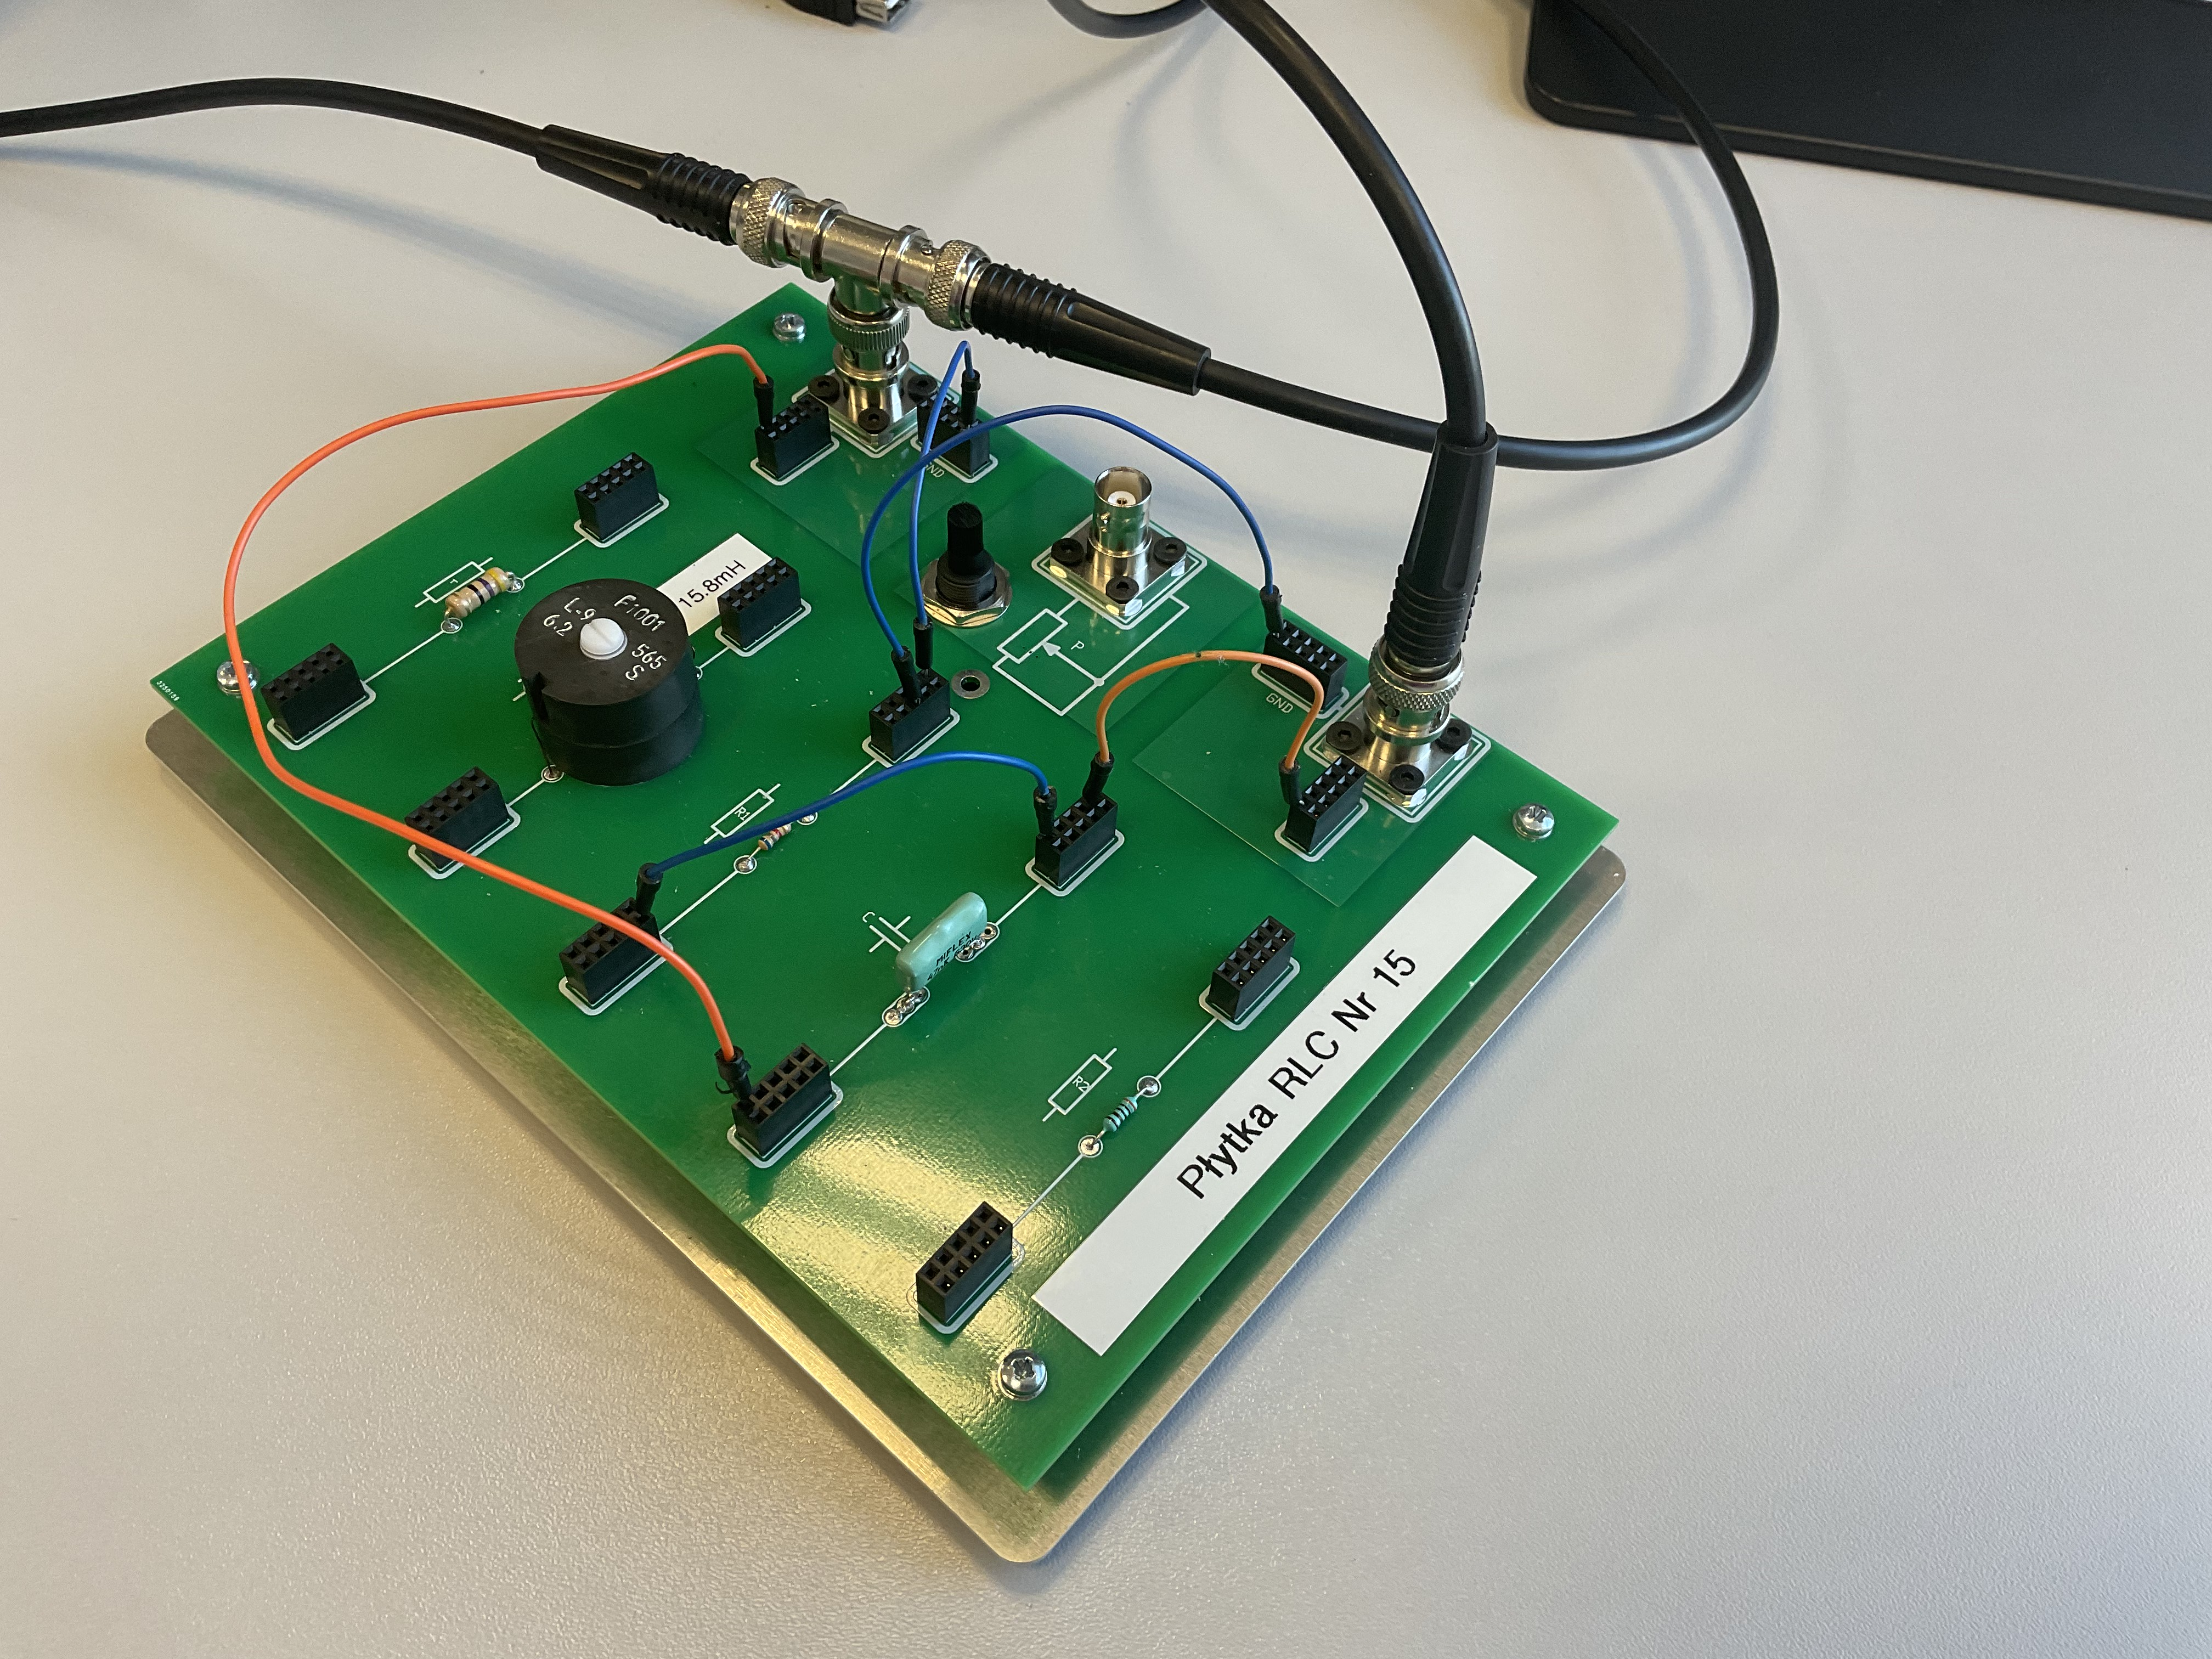
\includegraphics[width=7cm]{C0}}}%
    \qquad
    \subfloat[\centering ]{{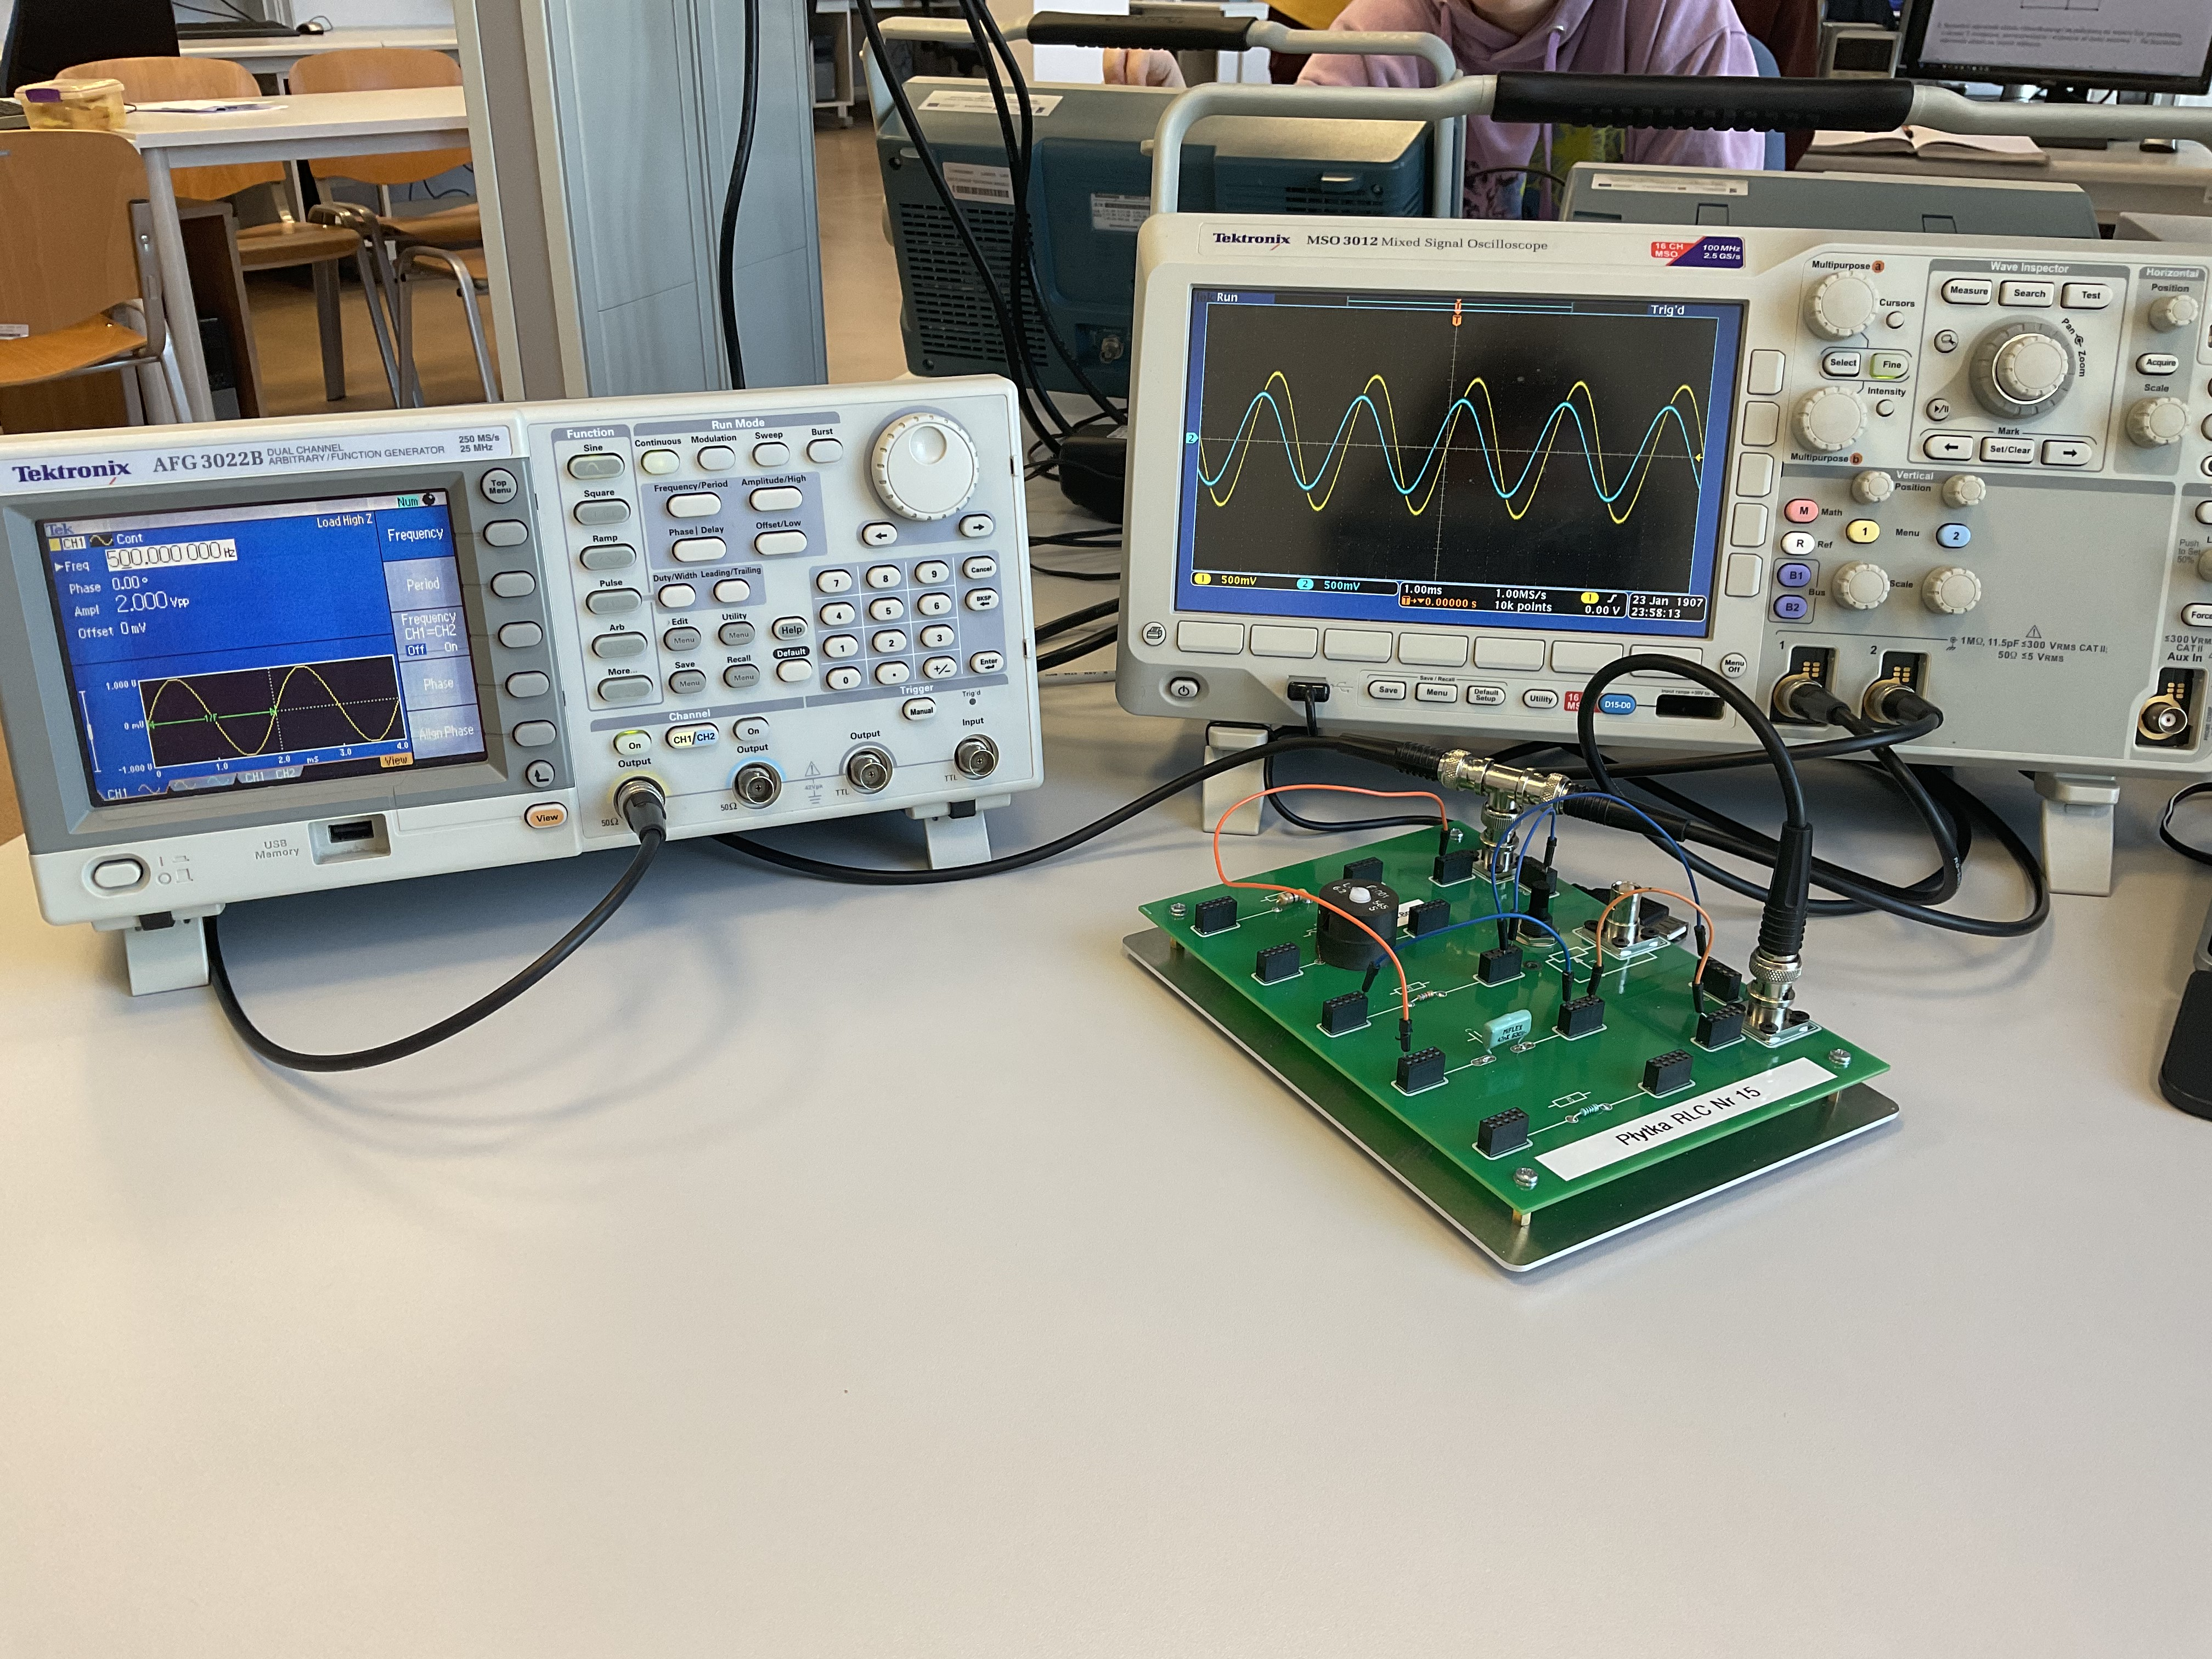
\includegraphics[width=7cm]{C1}}}%
\end{figure}

Montując układ CR użyłem rezystora o oporze $6.8 \ k \Omega$ oraz kondensatora o pojemności $47 \ nF$. Stała czasowa tego układu wynosi:
$$ \tau = RC = 6.8 \left[ k \Omega \right] \cdot 47 \left[ nF \right] = 6.8 \cdot 47 \cdot 10^3 \cdot 10^{-9} \left[ s \right] = 319.6 \cdot 10^{-6}  \left[ s \right] = 0.3196  \left[ ms \right] $$

Teoretyczna częstotliwość graniczna powinna więc wynosić:

$$ f_g = \frac{1}{2 \pi \tau} = \frac{1}{2 \pi \cdot 319.6} \cdot 10^{6} \left[ \frac{1}{s} \right] = 497.98  \left[ Hz \right] $$

Podałem na wejście układu sygnał sinusoidalny o apmlitudzie $2 \ V$pp o częstotliwościach od $30 \ Hz$ do $8 kHz$. Wartości amplitudy wyjściowej oraz przesunięcia fazowego wynosiły jak w tabeli poniżej: \\
\\

\begin{tabular}{ | m{4cm} | m{4cm}| m{4cm} | m{3.5cm} | } 
  \hline
  \textbf{Częstotliwość} & \textbf{Amplituda wyjściowa} & \textbf{Przesunięcie fazowe} & \textbf{Stosunek } $U_{WY} / U_{WE}$ \\ 
  \hline
  $30 \ Hz$ & $118 \ mV$ & $88.16^{\circ}$ & $0.059$ \\
  \hline
  $60 \ Hz$ & $228 \ mV$ & $86.34^{\circ}$ & $0.114$ \\
  \hline
  $120 \ Hz$ & $448 \ mV$ & $78.01^{\circ}$ & $0.224$ \\
  \hline
  $250 \ Hz$ & $800 \ mV$ & $63.8^{\circ}$ & $0.4$ \\
  \hline
  $500 \ Hz$ & $1.38 \ V$ & $46.37^{\circ}$ & $0.69$ \\
  \hline
  $1 \ kHz$ & $1.74 \ V$ & $26.54^{\circ}$ & $0.87$ \\
  \hline
  $2 \ kHz$ & $1.92 \ V$ & $14.83^{\circ}$ & $0.96$ \\
  \hline
  $4 \ kHz$ & $1.96 \ V$ & $7.159^{\circ}$ & $0.98$ \\
  \hline
  $8 \ kHz$ & $2 \ V$ & $2.882^{\circ}$ &  $1$\\
  \hline
\end{tabular}

\newpage
Zamieszczam poniżej odczyty oscyloskopu. Kanał 1 (żółty) - sygnał wejściowy, kanał 2 (niebieski) - sygnał wyjściowy.

\begin{figure}[H]
    \centering
    \subfloat[\centering $30 \ Hz$]{{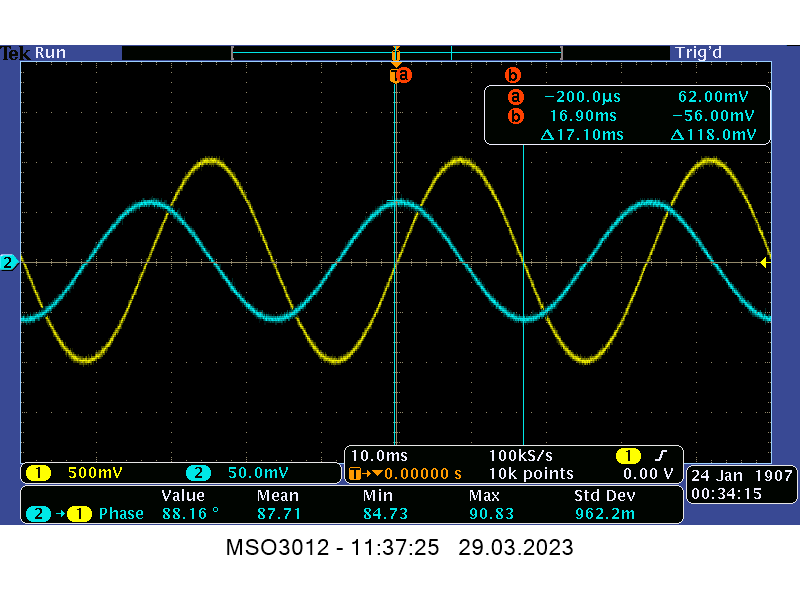
\includegraphics[width=7cm]{CR-30-Hz}}}%
    \qquad
    \subfloat[\centering $60 \ Hz$]{{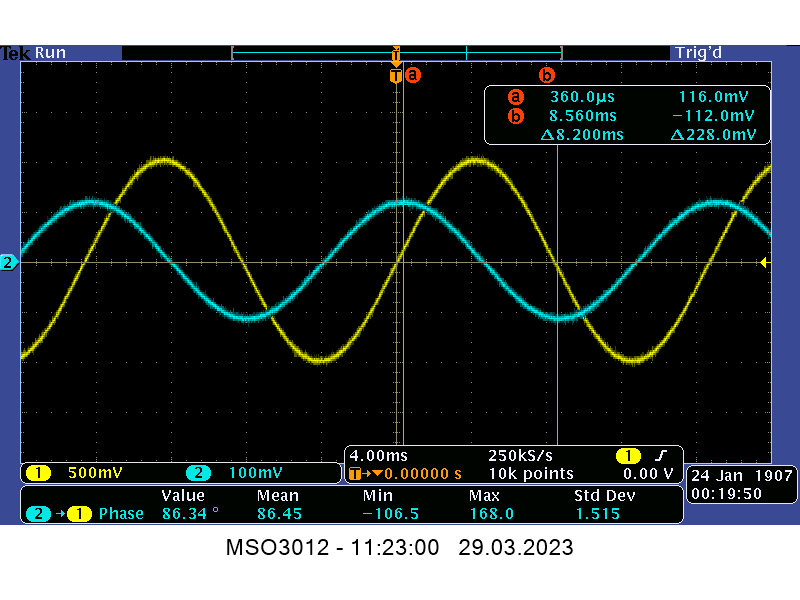
\includegraphics[width=7cm]{CR-60-Hz}}}%
\end{figure}

\begin{figure}[H]
    \centering
    \subfloat[\centering $120 \ Hz$]{{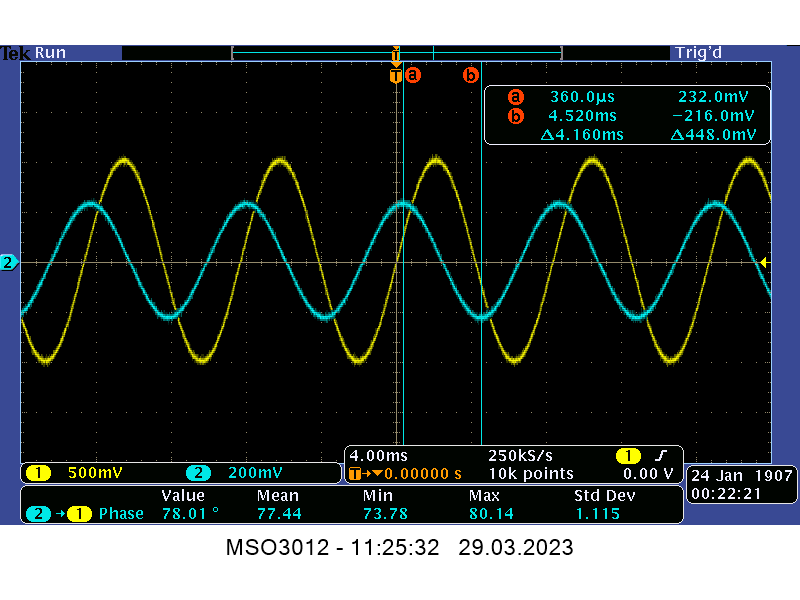
\includegraphics[width=7cm]{CR-120-Hz}}}%
    \qquad
    \subfloat[\centering $250 \ Hz$]{{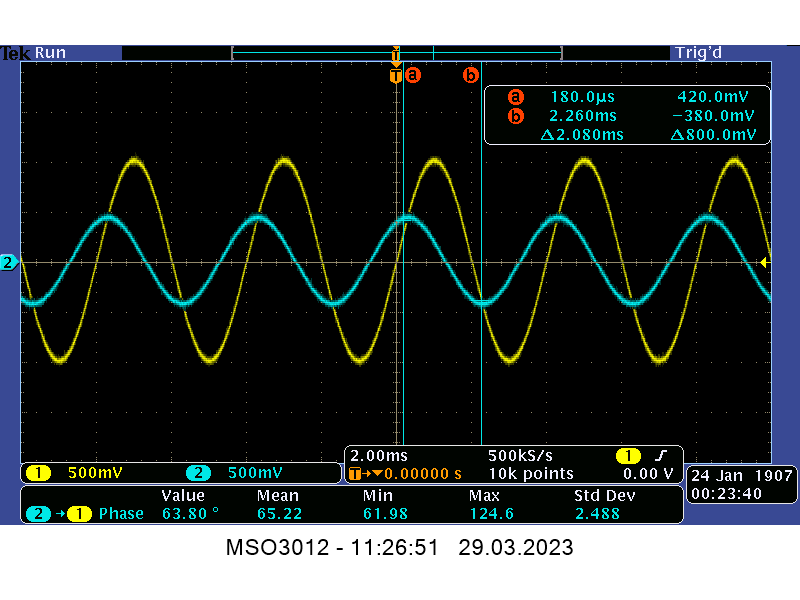
\includegraphics[width=7cm]{CR-250-Hz}}}%
\end{figure}

\begin{figure}[H]
    \centering
    \subfloat[\centering $500 \ Hz$]{{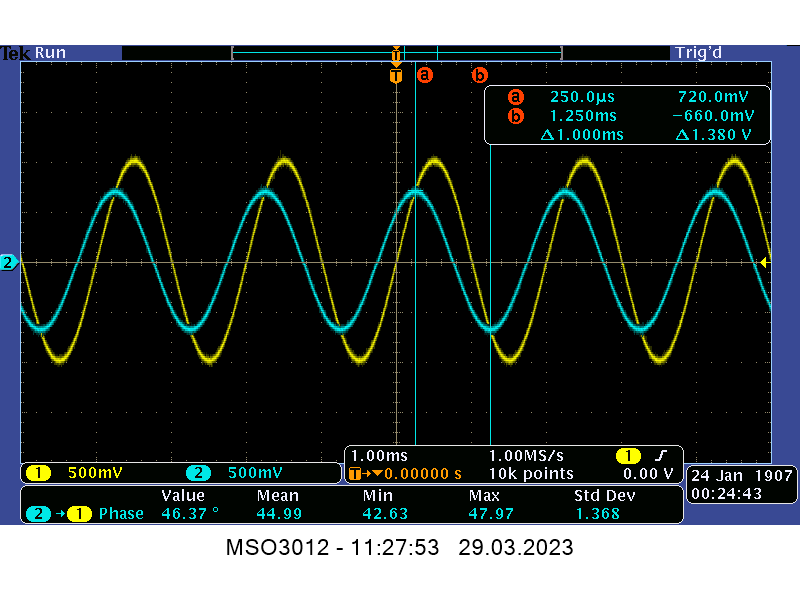
\includegraphics[width=7cm]{CR-500-Hz}}}%
    \qquad
    \subfloat[\centering $1 \ kHz$]{{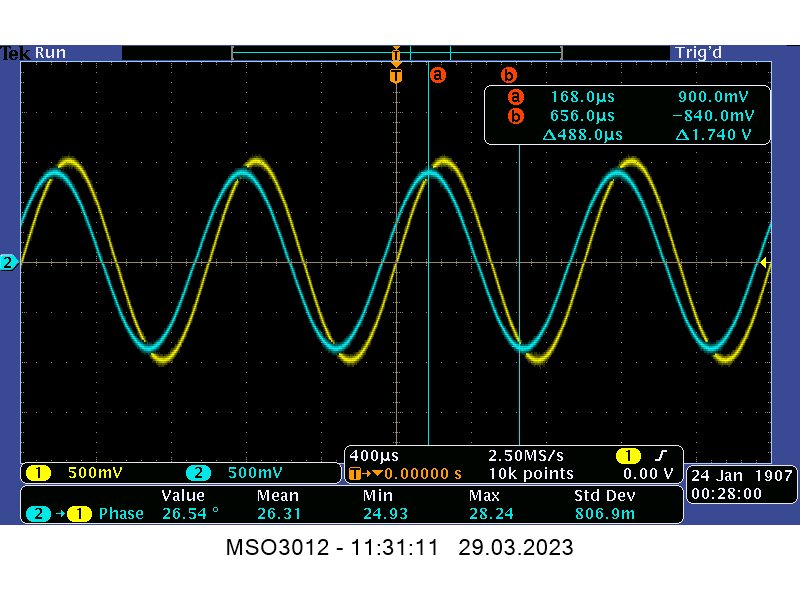
\includegraphics[width=7cm]{CR-1-kHz}}}%
\end{figure}

\begin{figure}[H]
    \centering
    \subfloat[\centering $2 \ kHz$]{{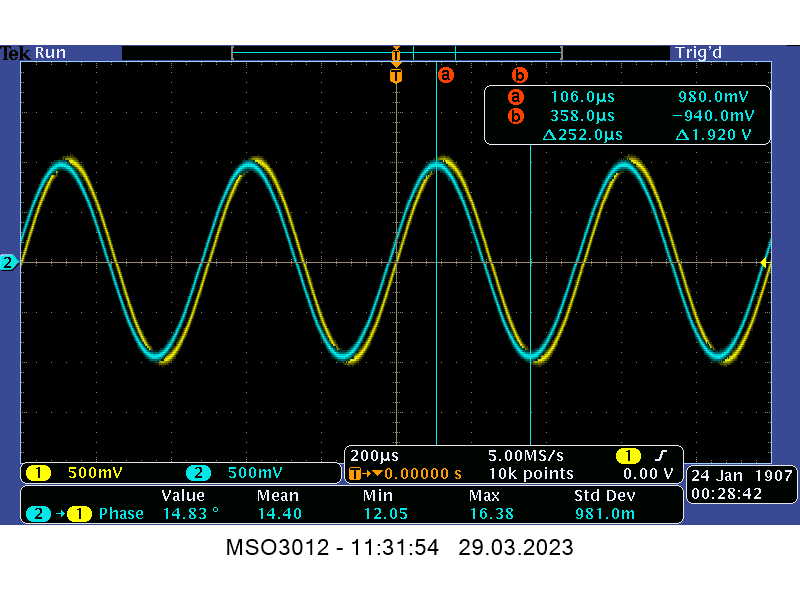
\includegraphics[width=7cm]{CR-2-kHz}}}%
    \qquad
    \subfloat[\centering $4 \ kHz$]{{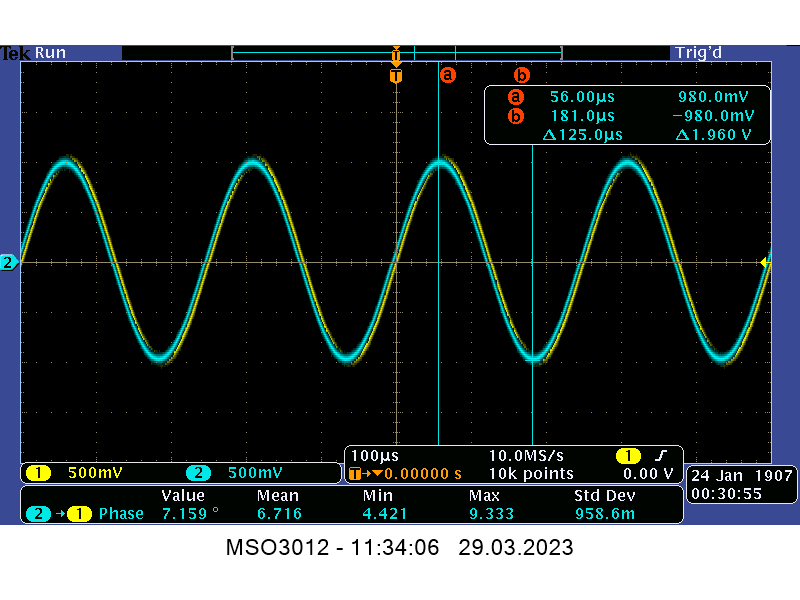
\includegraphics[width=7cm]{CR-4-kHz}}}%
\end{figure}

\begin{figure}[H]
    \centering
    \subfloat[\centering $8 \ kHz$]{{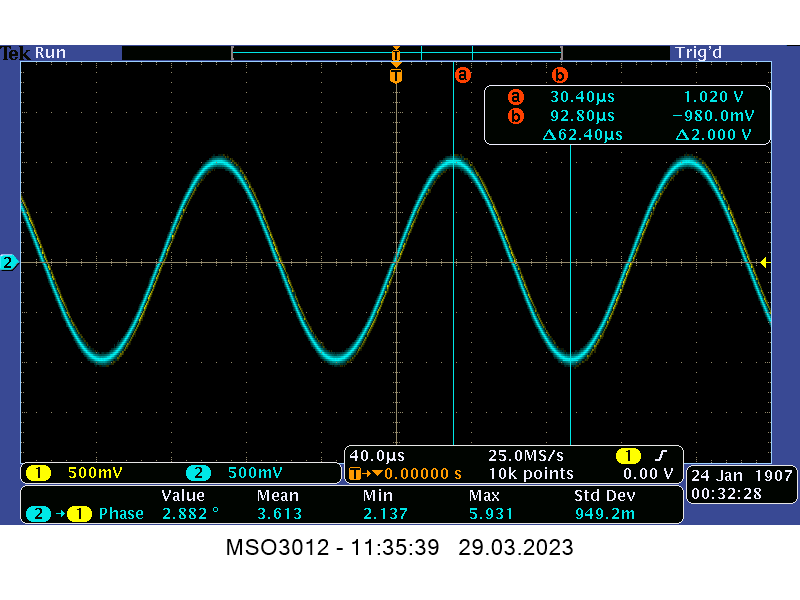
\includegraphics[width=7cm]{CR-8-kHz}}}%
\end{figure}

\newpage
Wykresy: stosunek $U_{WY} / U_{WE}$ oraz przesunięcie fazowe w zależności od częstotliwości sygnału.

\begin{figure}[H]
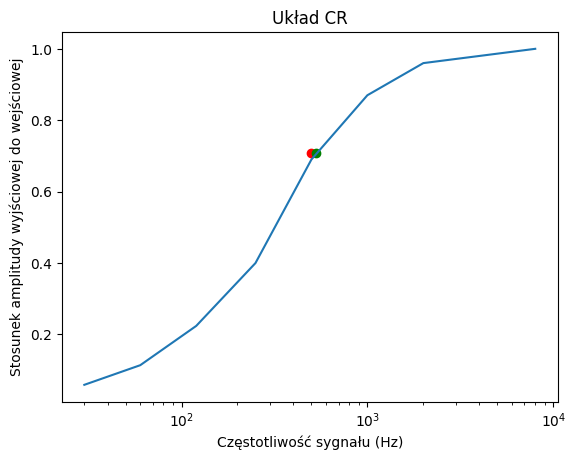
\includegraphics[scale=0.7]{D0}
\centering
\captionsetup{labelformat=empty}
\caption{}
\end{figure}

\begin{figure}[H]
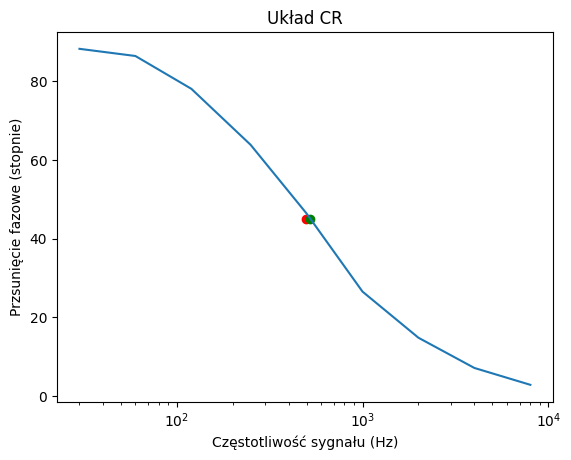
\includegraphics[scale=0.7]{D1}
\centering
\captionsetup{labelformat=empty}
\caption{}
\end{figure}

\newpage
\paragraph{Ćwiczenie 2.2\\}
Badanie odpowiedzi układu różniczkującego na podawaną na wejście falę prostokątną okresie $T$ mniejszym, porównywalnym i większym od stałej czasowej $\tau$. Badanie odpowiedzi układu na impuls trójkątny. \\

\begin{figure}[H]
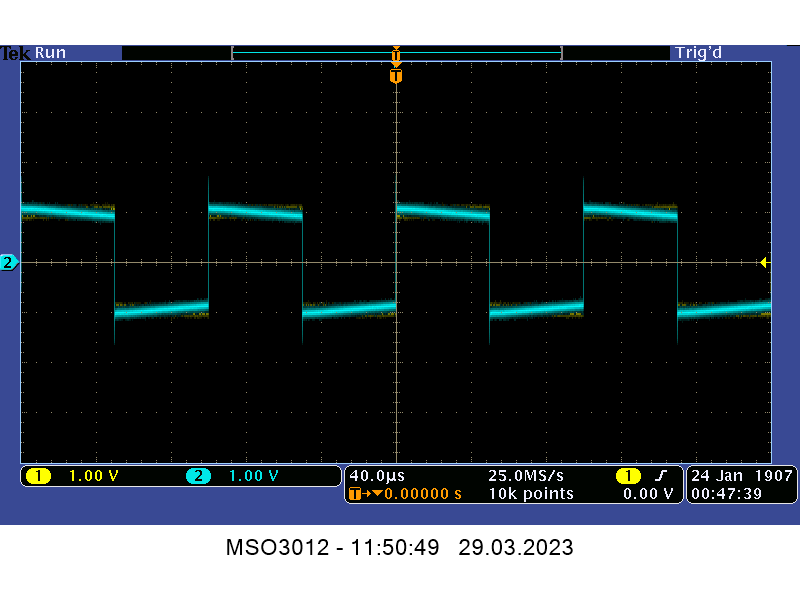
\includegraphics[scale=0.65]{CR-square-0_1ms}
\centering
\captionsetup{labelformat=empty}
\caption{Sygnał prostokątny \ \ $T = 0.1 \ ms \ \ \ f = 10 \ kHz$}
\end{figure}

\begin{figure}[H]
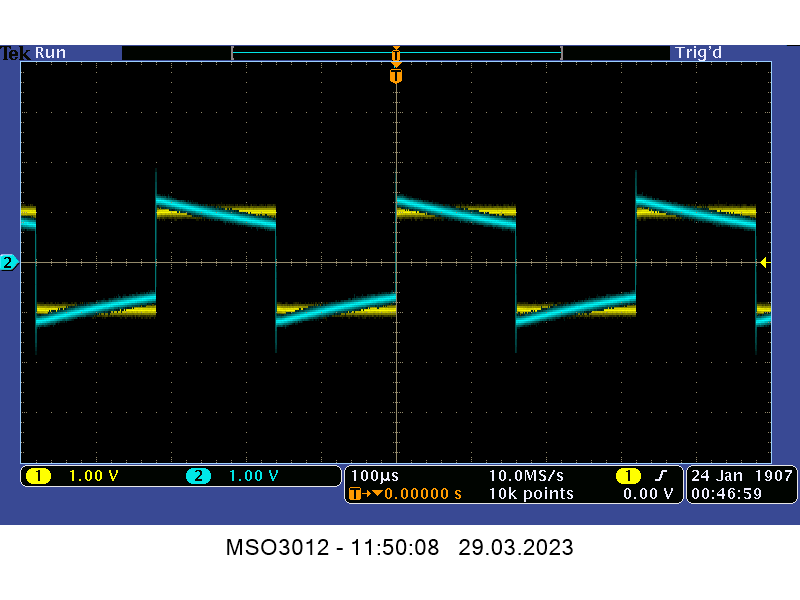
\includegraphics[scale=0.65]{CR-square-0_32ms}
\centering
\captionsetup{labelformat=empty}
\caption{Sygnał prostokątny \ \ $T = 0.32 \ ms \ \ \ f = 3.125 \ kHz$}
\end{figure}

\begin{figure}[H]
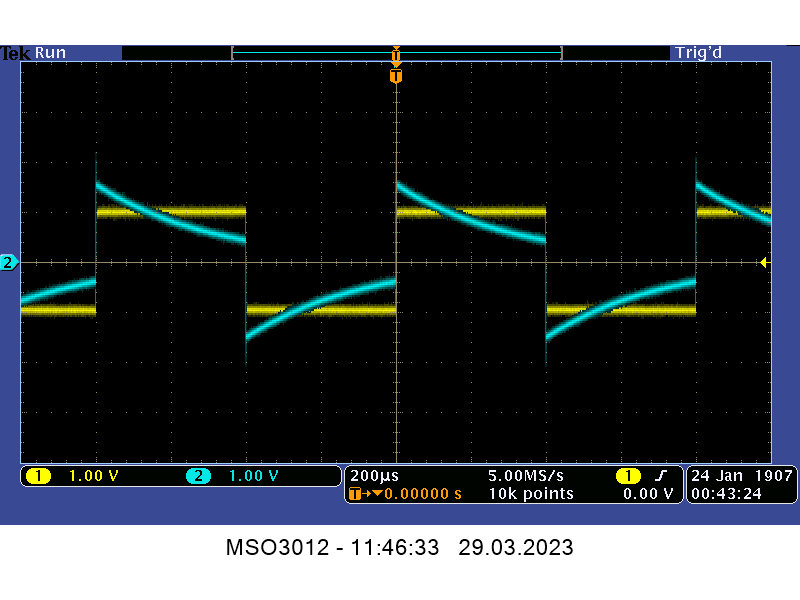
\includegraphics[scale=0.65]{CR-square-0_8ms}
\centering
\captionsetup{labelformat=empty}
\caption{Sygnał prostokątny \ \ $T = 0.8 \ ms \ \ \ f = 1.25 \ kHz$}
\end{figure}

\begin{figure}[H]
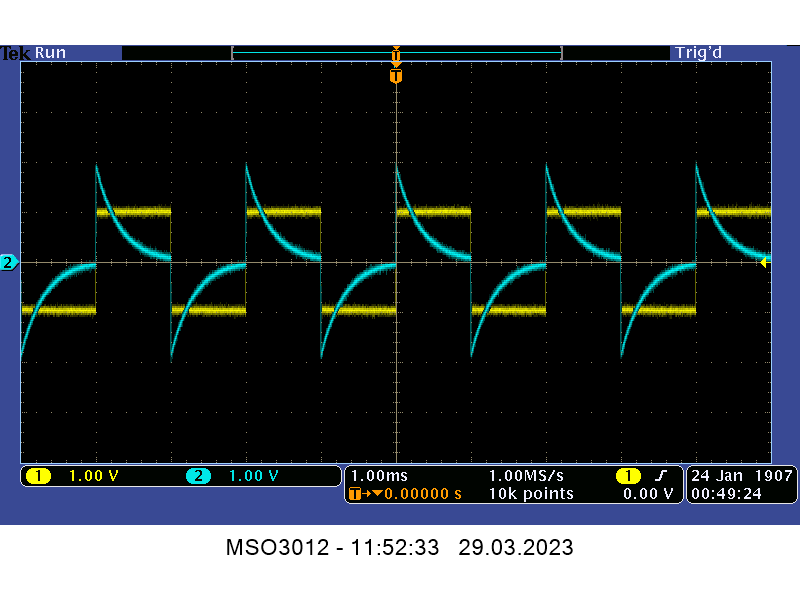
\includegraphics[scale=0.65]{CR-square-2ms}
\centering
\captionsetup{labelformat=empty}
\caption{Sygnał prostokątny \ \ $T = 2 \ ms \ \ \ f = 500 \ Hz$}
\end{figure}

\begin{figure}[H]
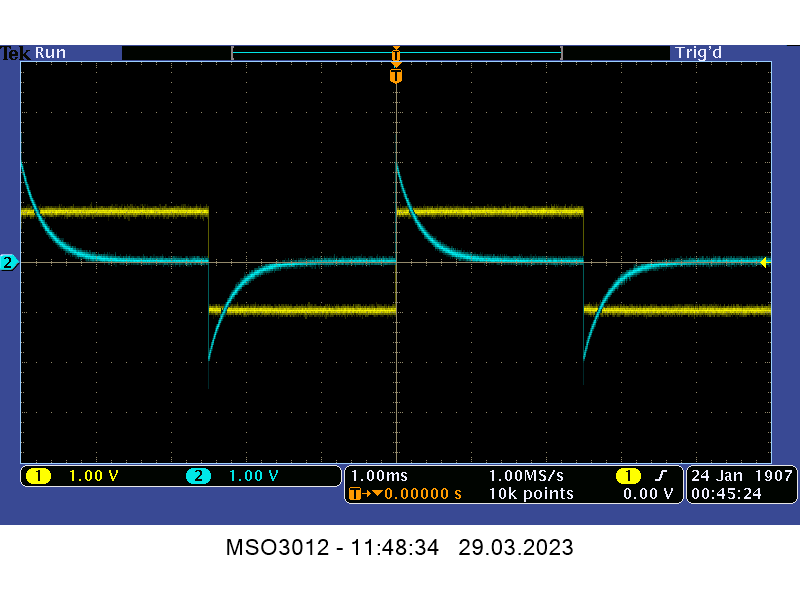
\includegraphics[scale=0.65]{CR-square-5ms}
\centering
\captionsetup{labelformat=empty}
\caption{Sygnał prostokątny \ \ $T = 5 \ ms \ \ \ f = 200 \ Hz$}
\end{figure}

\begin{figure}[H]
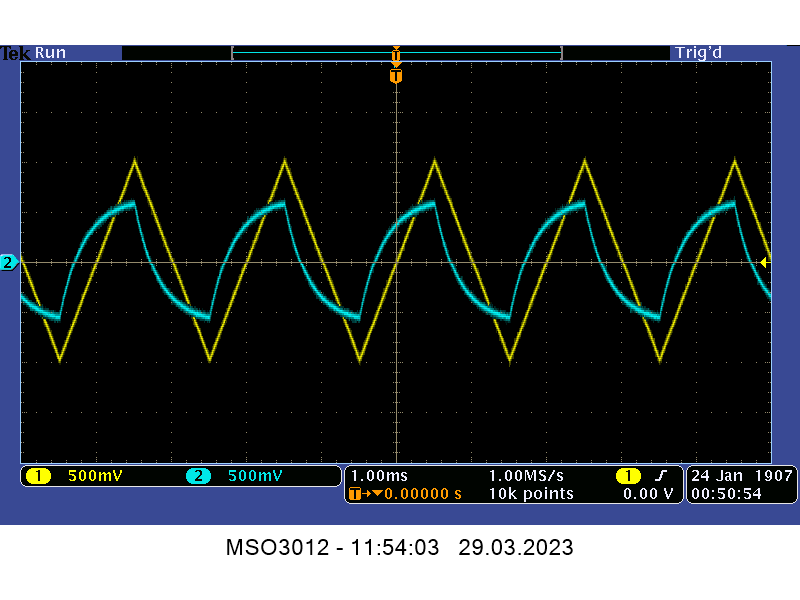
\includegraphics[scale=0.65]{CR-triangle}
\centering
\captionsetup{labelformat=empty}
\caption{Sygnał trójkątny \ \ $T = 2 \ ms \ \ \ f = 500 \ Hz$}
\end{figure}



\newpage
\paragraph{Ćwiczenie 2.3\\}
Zmontowanie układu całkujacego, zmierzenie stosunku amplitudy sygnału wejściowego do wyjściowego oraz kąta przesunięcia fazowego w zależności od częstotliwości. Przedstawienie tych wartości na wykresie i wyznaczenie dolnej częstotliwości granicznej.

\begin{figure}[H]
    \centering
    \subfloat[\centering ]{{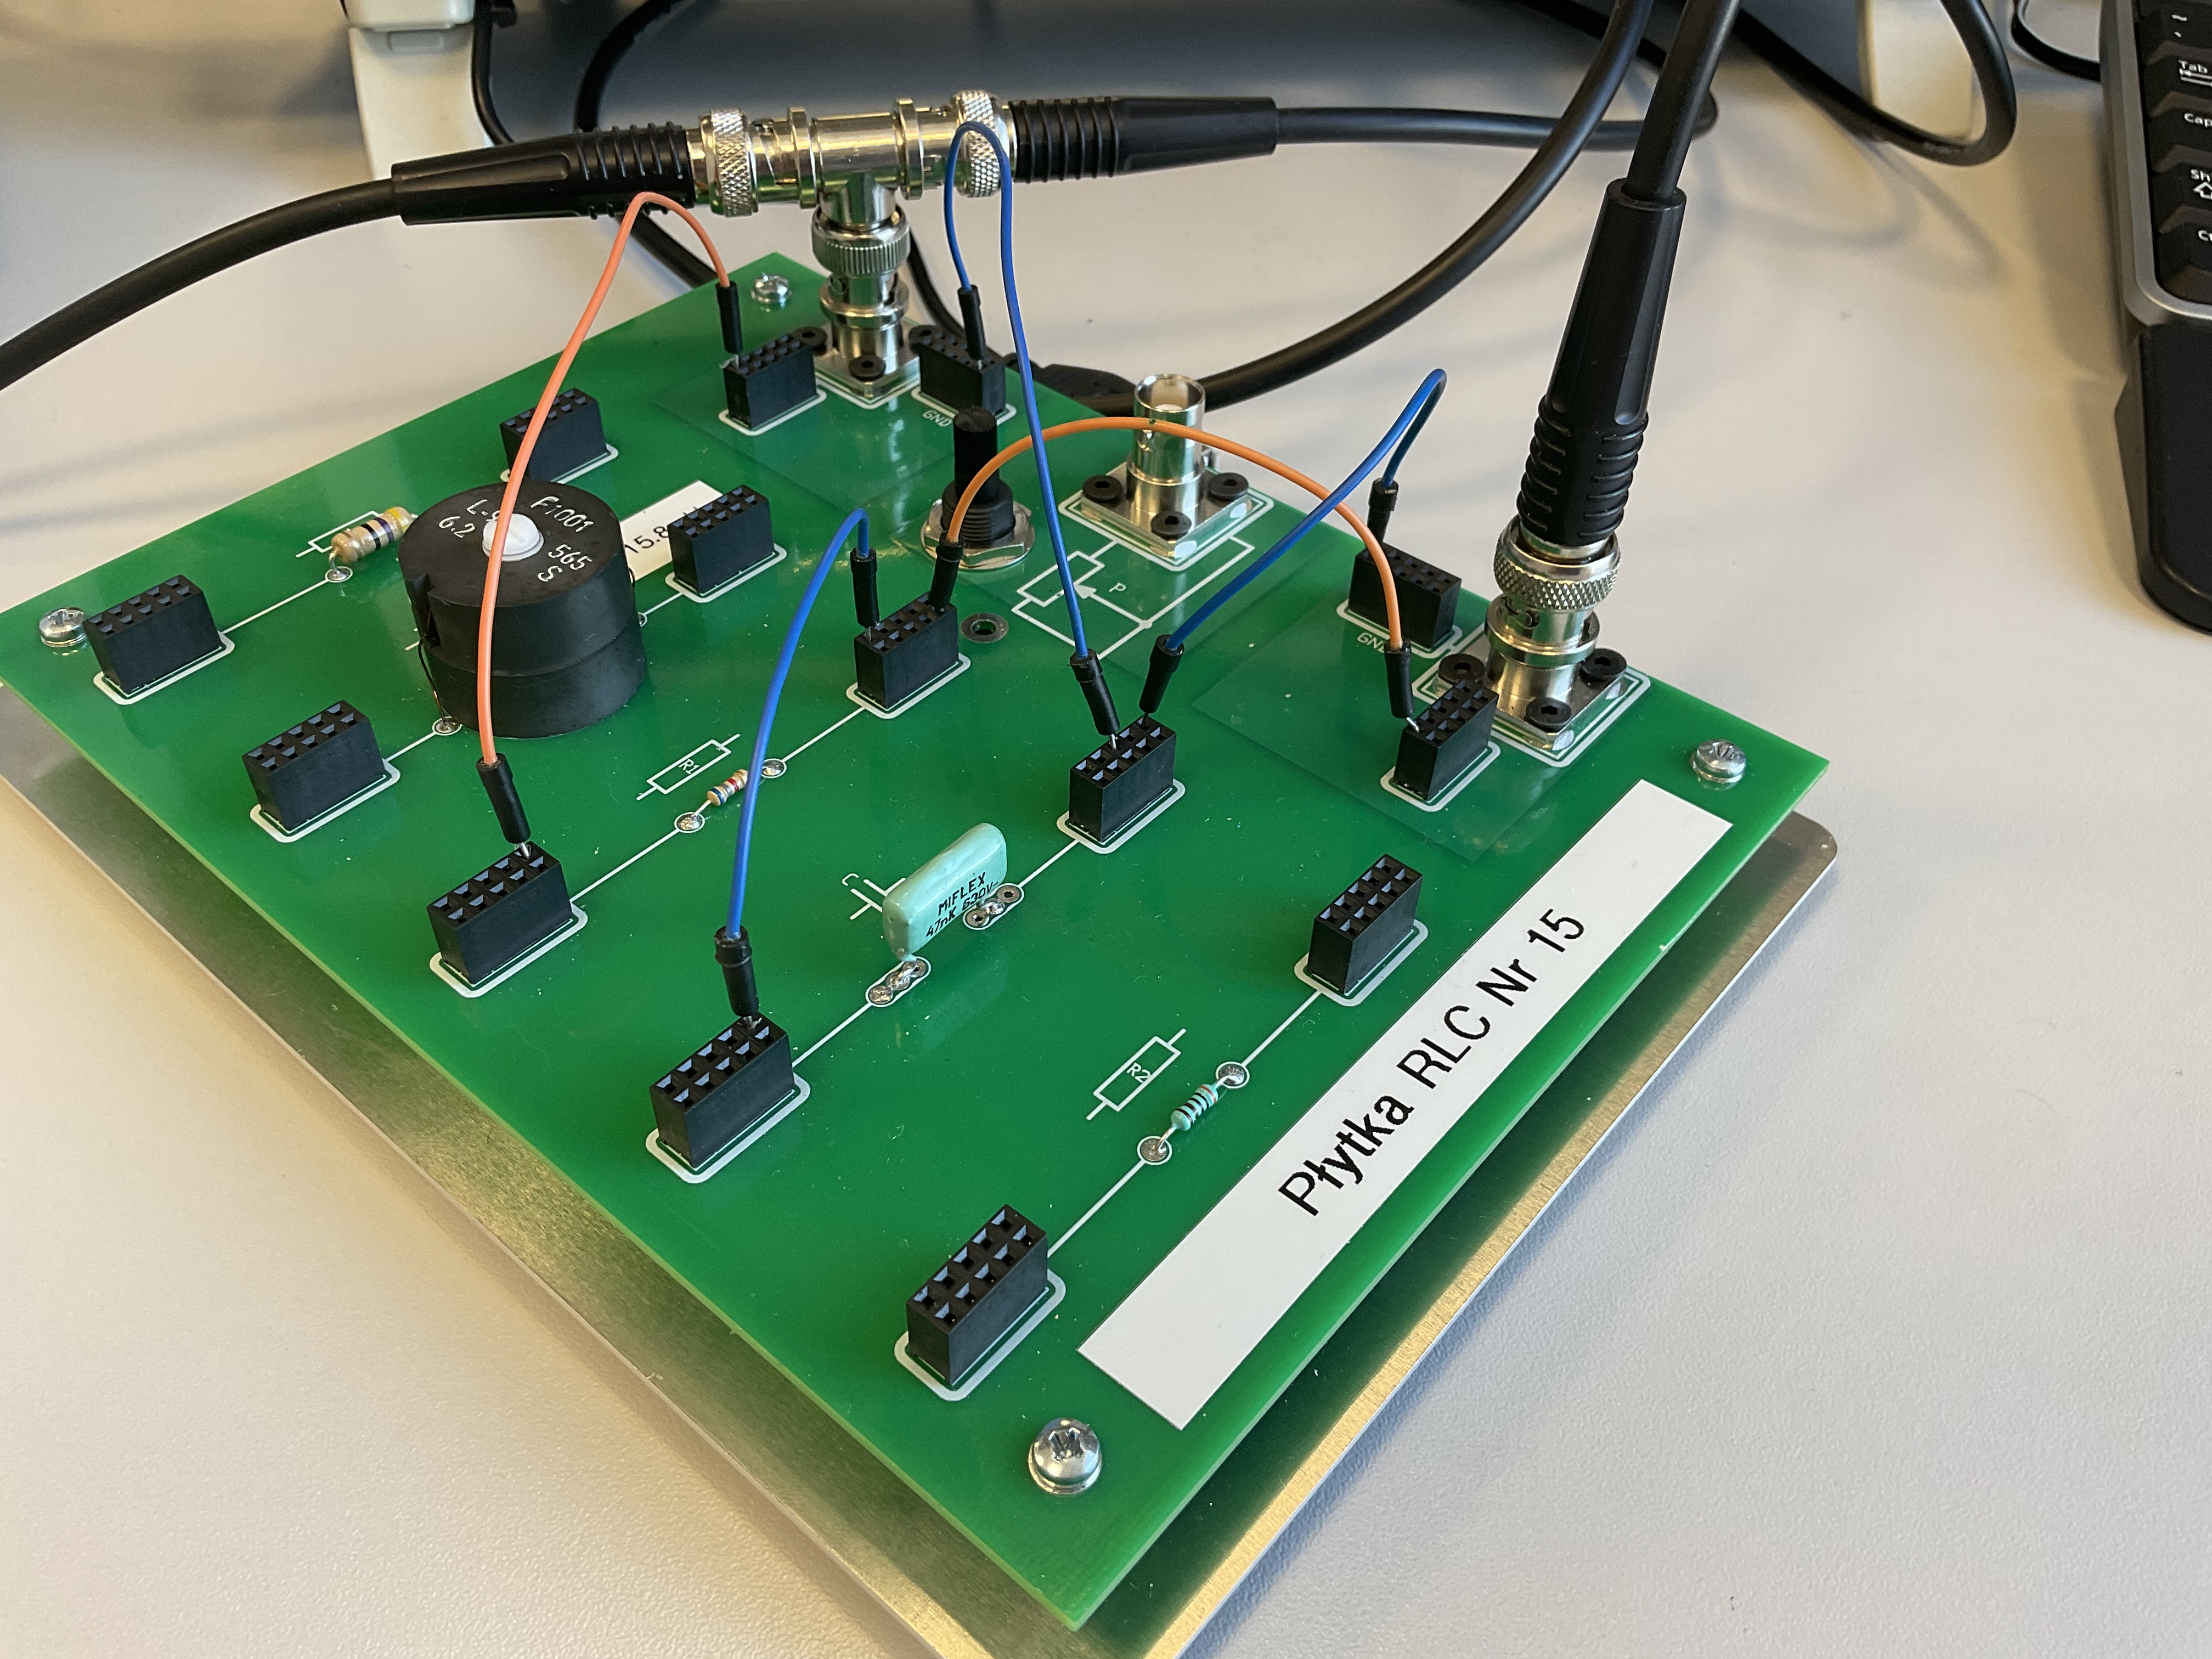
\includegraphics[width=7cm]{C3}}}%
    \qquad
    \subfloat[\centering ]{{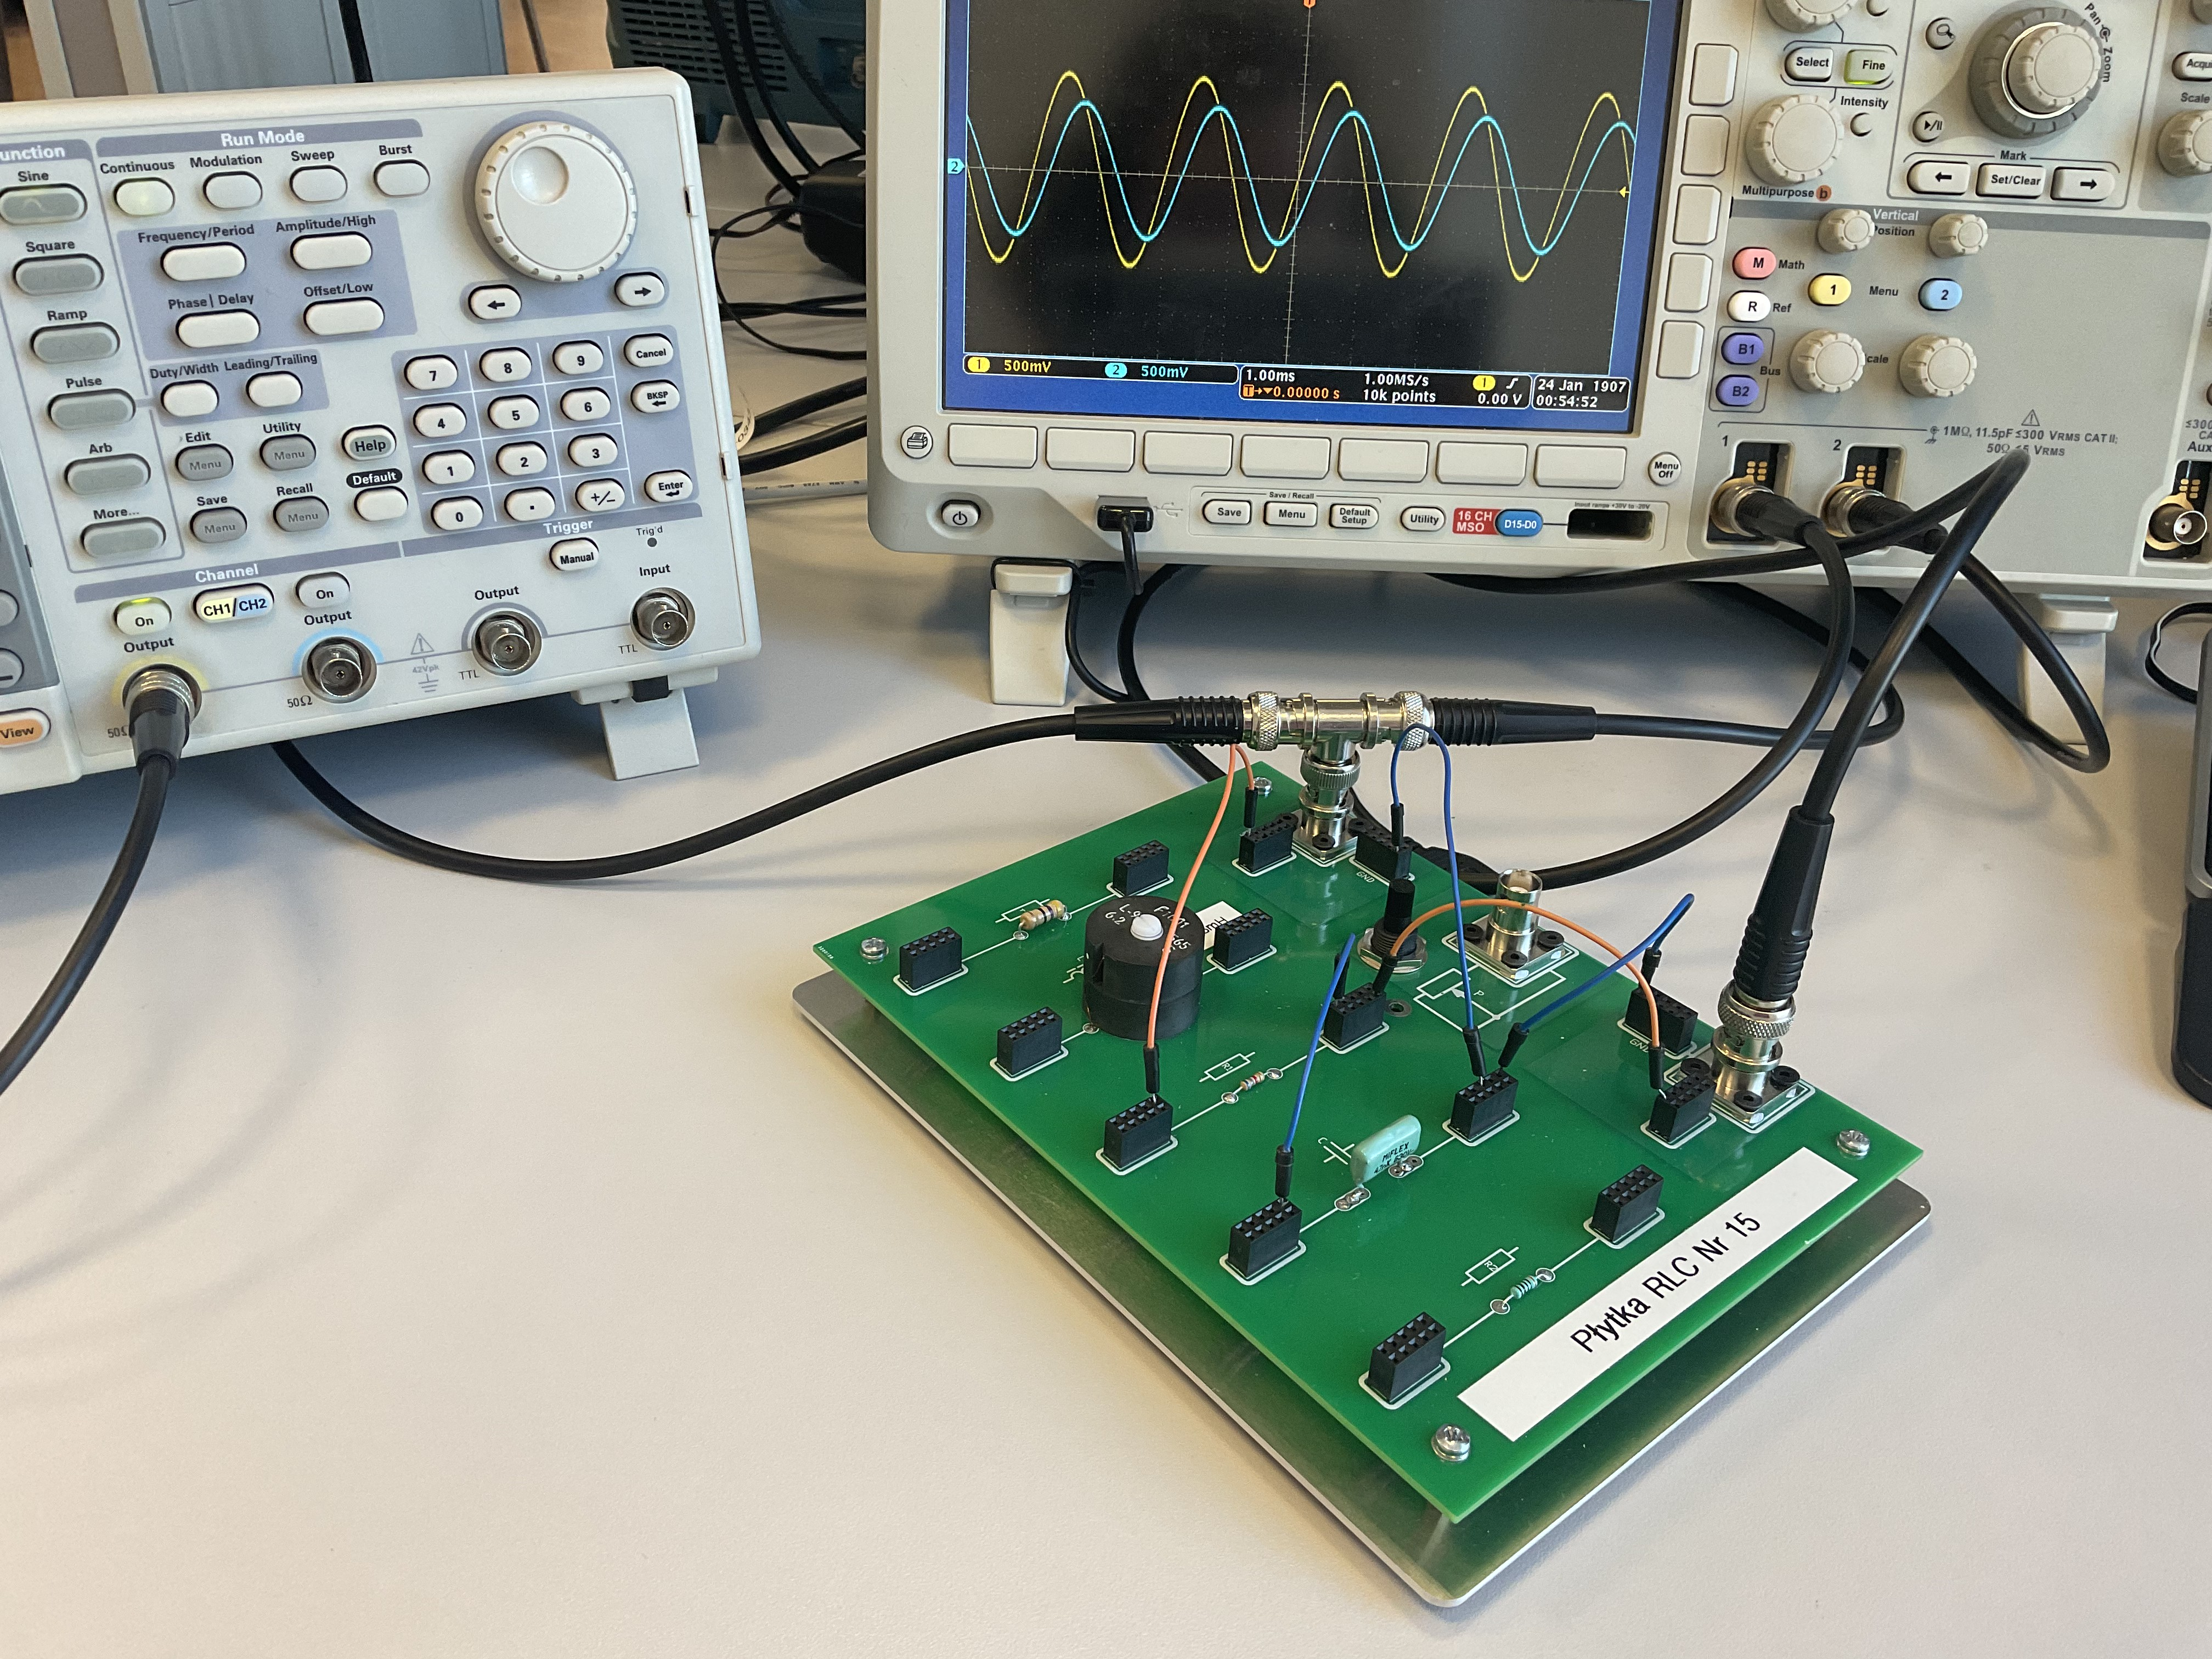
\includegraphics[width=7cm]{C2}}}%
\end{figure}

Montując układ RC użyłem tych samych komponentów co w poprzednim ćwiczeniu. Stała czasowa oraz częstotliwość graniczna tego układu wynoszą tyle samo co w Ćwiczeniu 2.1:
$$ \tau = RC = 0.3196  \left[ ms \right] $$
$$ f_g = 497.98  \left[ Hz \right] $$

Podałem na wejście układu sygnał sinusoidalny o apmlitudzie $2 \ V$pp o częstotliwościach od $30 \ Hz$ do $8 kHz$. Wartości amplitudy wyjściowej oraz przesunięcia fazowego wynosiły jak w tabeli poniżej: \\
\\

\begin{tabular}{ | m{4cm} | m{4cm}| m{4cm} | m{3.5cm} | } 
  \hline
  \textbf{Częstotliwość} & \textbf{Amplituda wyjściowa} & \textbf{Przesunięcie fazowe} & \textbf{Stosunek } $U_{WY} / U_{WE}$ \\ 
  \hline
  $30 \ Hz$ & $2 \ V$ & $-1.884^{\circ}$ & $1$ \\
  \hline
  $60 \ Hz$ & $1.98 \ V$ & $-7.63^{\circ}$ & $0.99$ \\
  \hline
  $120 \ Hz$ & $1.92 \ V$ & $-13.72^{\circ}$ & $0.96$ \\
  \hline
  $250 \ Hz$ & $1.76 \ V$ & $-26.25^{\circ}$ & $0.88$ \\
  \hline
  $500 \ Hz$ & $1.38 \ V$ & $-45.66^{\circ}$ & $0.68$ \\
  \hline
  $1 \ kHz$ & $860 \ mV$ & $-64.7^{\circ}$ & $0.43$ \\
  \hline
  $2 \ kHz$ & $488 \ mV$ & $-73.21^{\circ}$ & $0.244$ \\
  \hline
  $4 \ kHz$ & $256 \ mV$ & $-81.74^{\circ}$ & $0.128$ \\
  \hline
  $8 \ kHz$ & $126 \ mV$ & $-86.59^{\circ}$ &  $0.063$ \\
  \hline
\end{tabular}

\newpage
Odczyty oscyloskopu. 

\begin{figure}[H]
    \centering
    \subfloat[\centering $30 \ Hz$]{{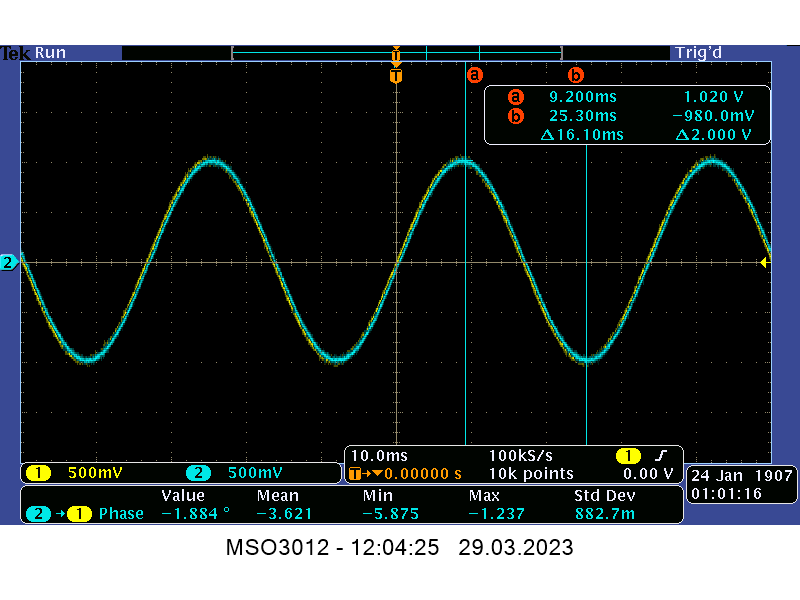
\includegraphics[width=7cm]{RC-30-Hz}}}%
    \qquad
    \subfloat[\centering $60 \ Hz$]{{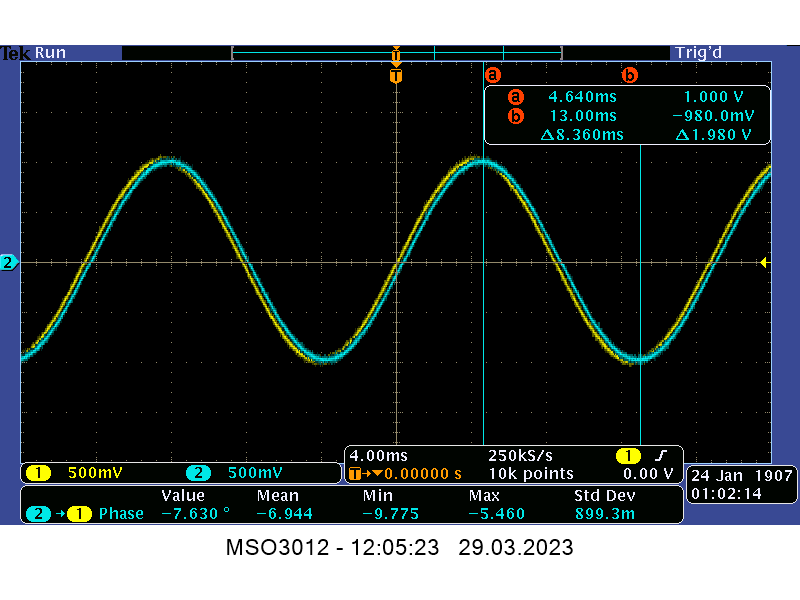
\includegraphics[width=7cm]{RC-60-Hz}}}%
\end{figure}

\begin{figure}[H]
    \centering
    \subfloat[\centering $120 \ Hz$]{{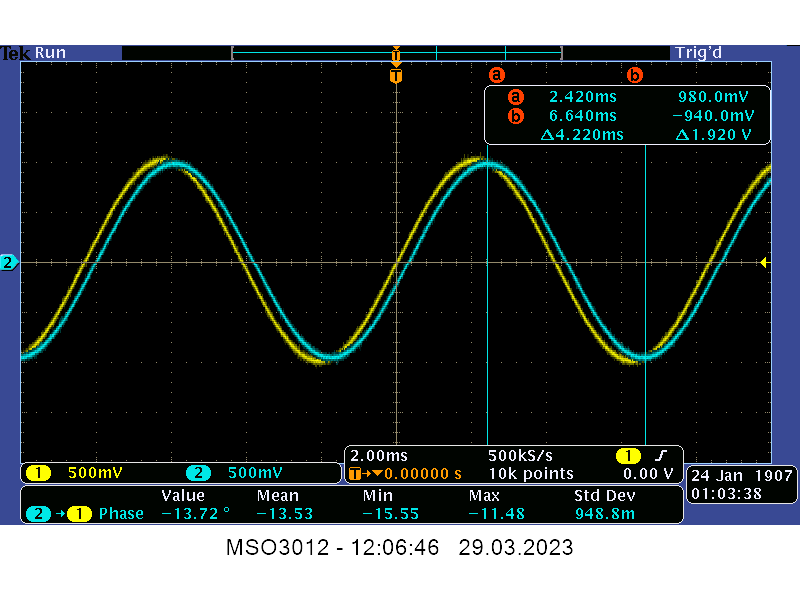
\includegraphics[width=7cm]{RC-120-Hz}}}%
    \qquad
    \subfloat[\centering $250 \ Hz$]{{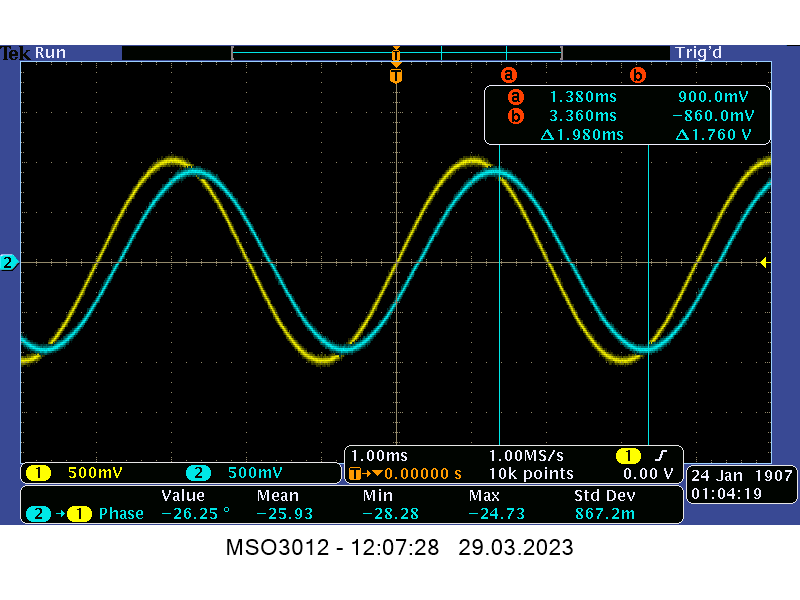
\includegraphics[width=7cm]{RC-250-Hz}}}%
\end{figure}

\begin{figure}[H]
    \centering
    \subfloat[\centering $500 \ Hz$]{{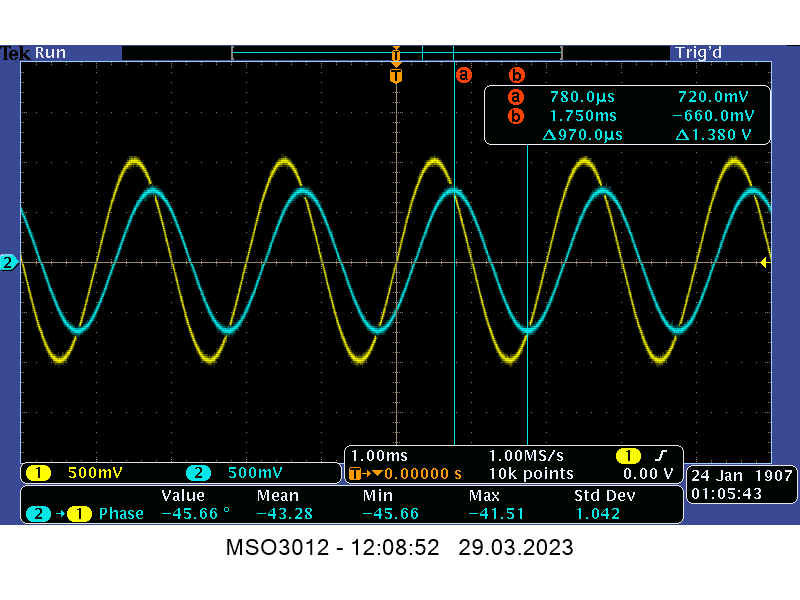
\includegraphics[width=7cm]{RC-500-Hz}}}%
    \qquad
    \subfloat[\centering $1 \ kHz$]{{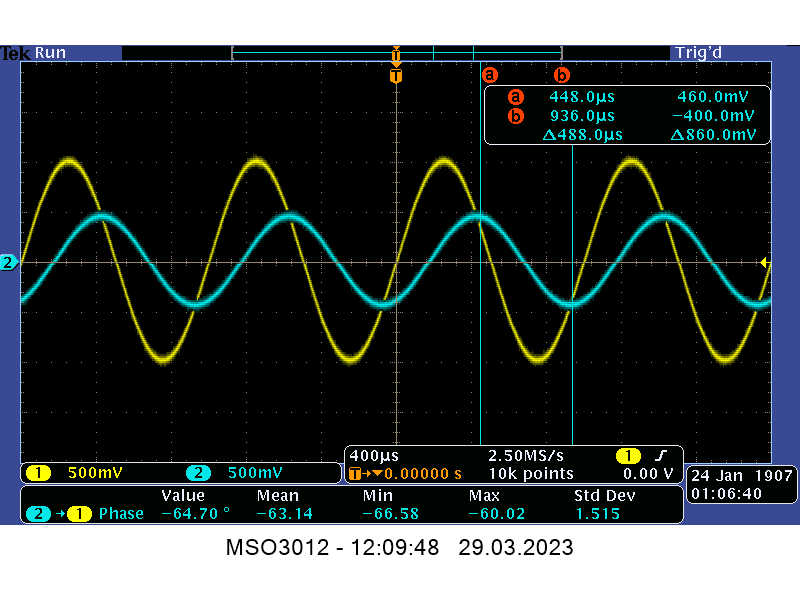
\includegraphics[width=7cm]{RC-1-kHz}}}%
\end{figure}

\begin{figure}[H]
    \centering
    \subfloat[\centering $2 \ kHz$]{{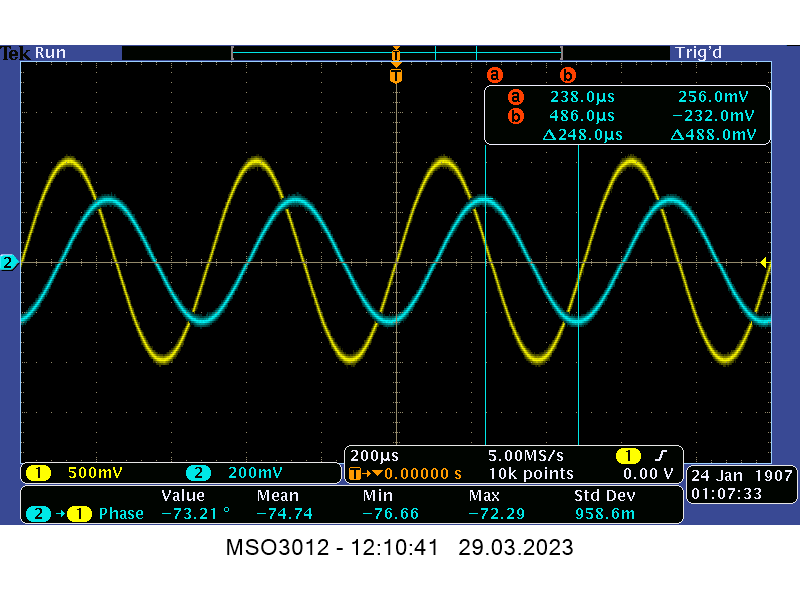
\includegraphics[width=7cm]{RC-2-kHz}}}%
    \qquad
    \subfloat[\centering $4 \ kHz$]{{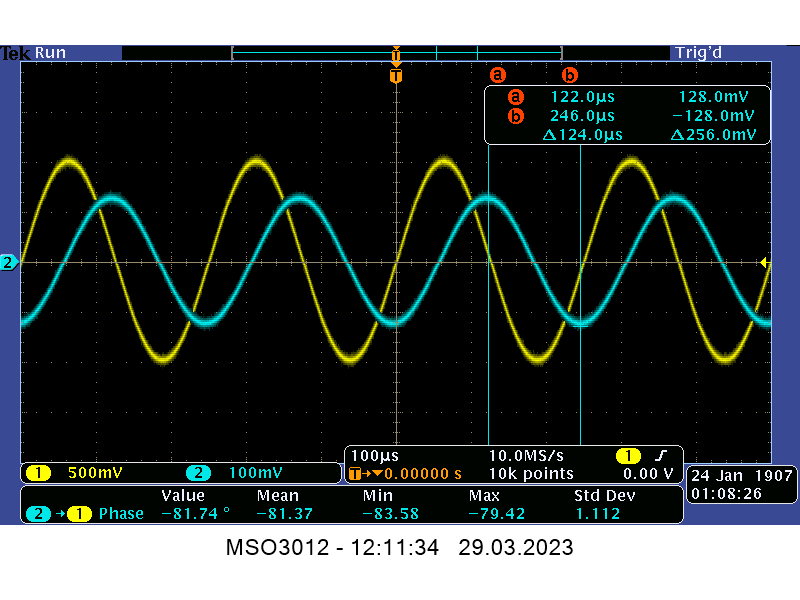
\includegraphics[width=7cm]{RC-4-kHz}}}%
\end{figure}

\begin{figure}[H]
    \centering
    \subfloat[\centering $8 \ kHz$]{{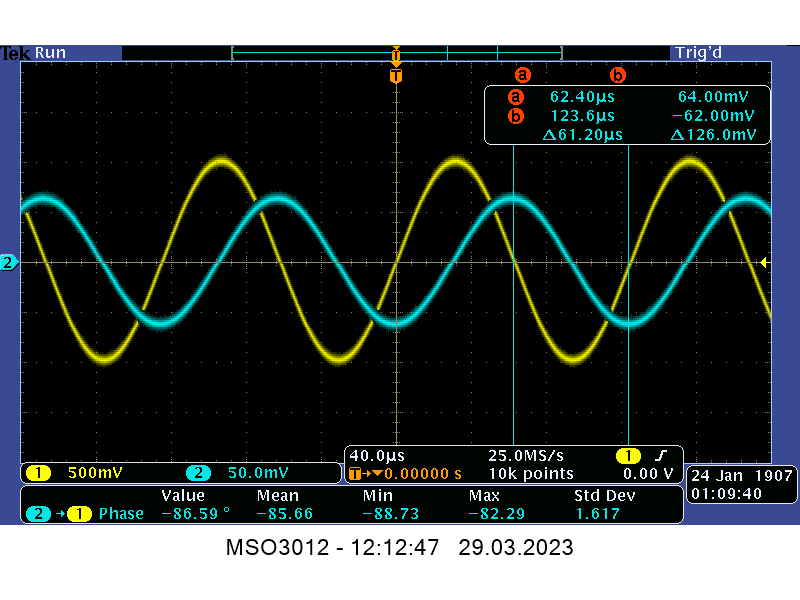
\includegraphics[width=7cm]{RC-8-kHz}}}%
\end{figure}

\newpage
Wykresy: stosunek $U_{WY} / U_{WE}$ oraz przesunięcie fazowe w zależności od częstotliwości sygnału.

\begin{figure}[H]
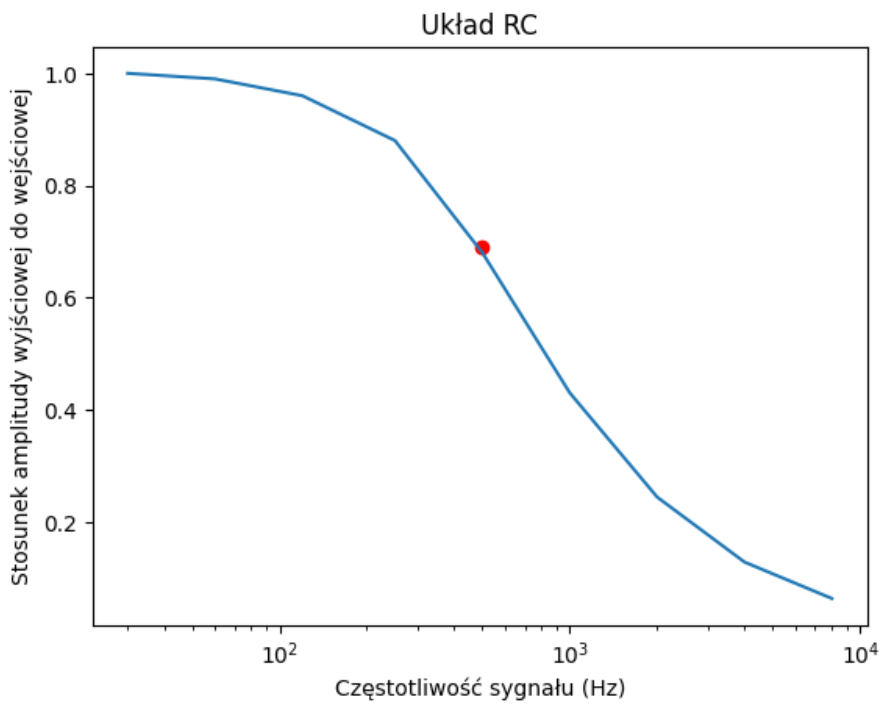
\includegraphics[scale=0.7]{D2}
\centering
\captionsetup{labelformat=empty}
\caption{}
\end{figure}

\begin{figure}[H]
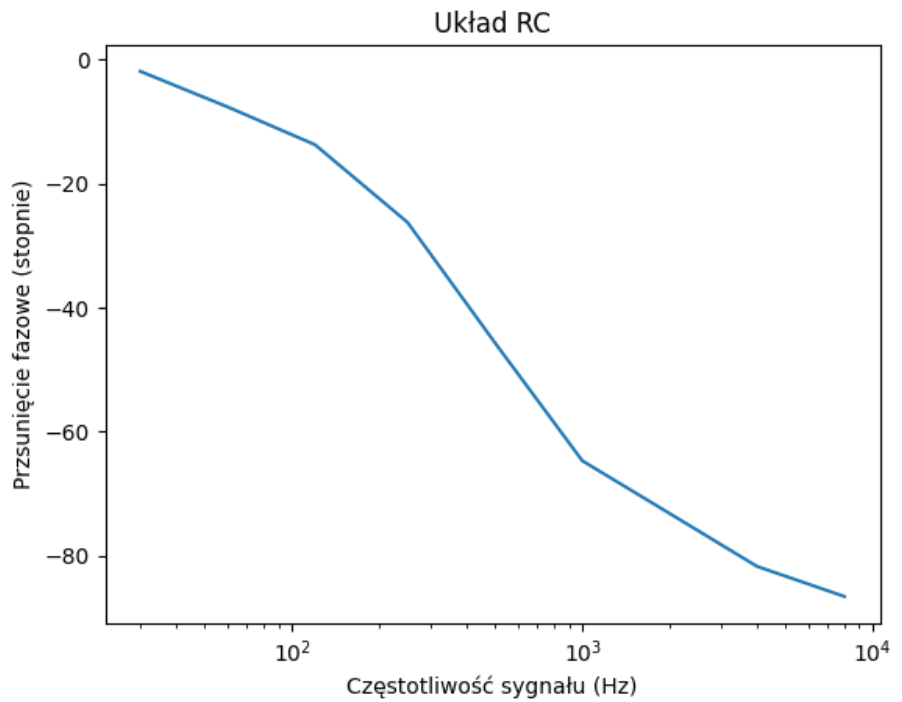
\includegraphics[scale=0.7]{D3}
\centering
\captionsetup{labelformat=empty}
\caption{}
\end{figure}

\newpage
Podanie na wejście układu RC fali prostokątnej o okresach z zakresu od $0.5 \tau$ do $10 \tau$. Obserwacja przebiegów impulsów wyjściowych.

\begin{figure}[H]
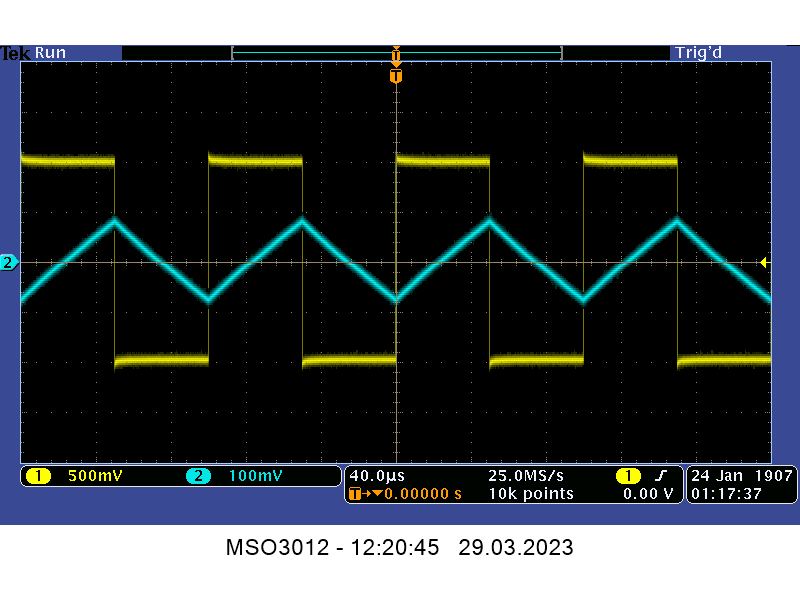
\includegraphics[scale=0.65]{RC-square-0_1ms}
\centering
\captionsetup{labelformat=empty}
\caption{Sygnał prostokątny \ \ $T = 0.1 \ ms \ \ \ f = 10 \ kHz$}
\end{figure}

\begin{figure}[H]
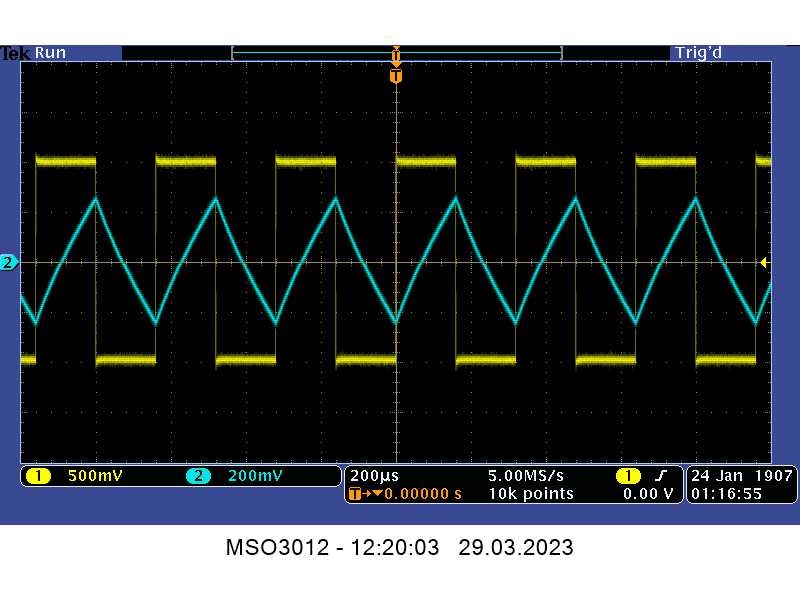
\includegraphics[scale=0.65]{RC-square-0_32ms}
\centering
\captionsetup{labelformat=empty}
\caption{Sygnał prostokątny \ \ $T = 0.32 \ ms \ \ \ f = 3.125 \ kHz$}
\end{figure}

\begin{figure}[H]
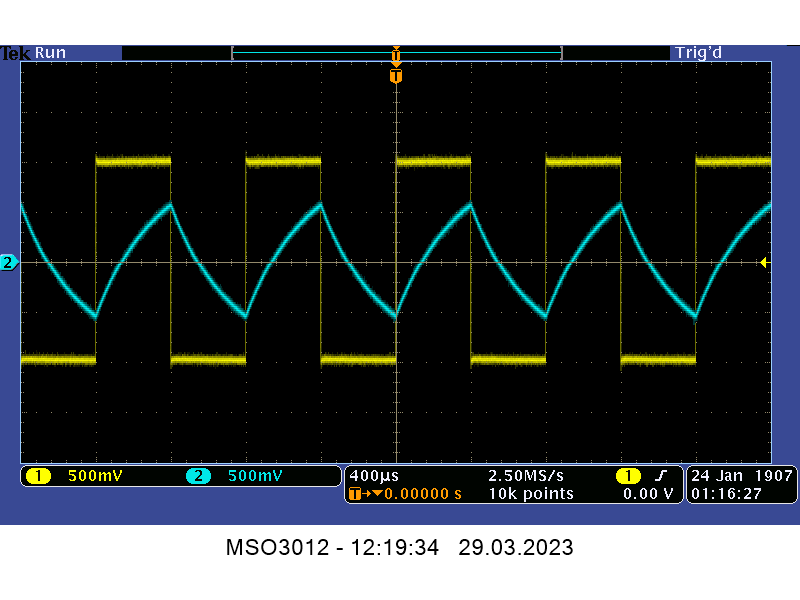
\includegraphics[scale=0.65]{RC-square-0_8ms}
\centering
\captionsetup{labelformat=empty}
\caption{Sygnał prostokątny \ \ $T = 0.8 \ ms \ \ \ f = 1.25 \ kHz$}
\end{figure}

\begin{figure}[H]
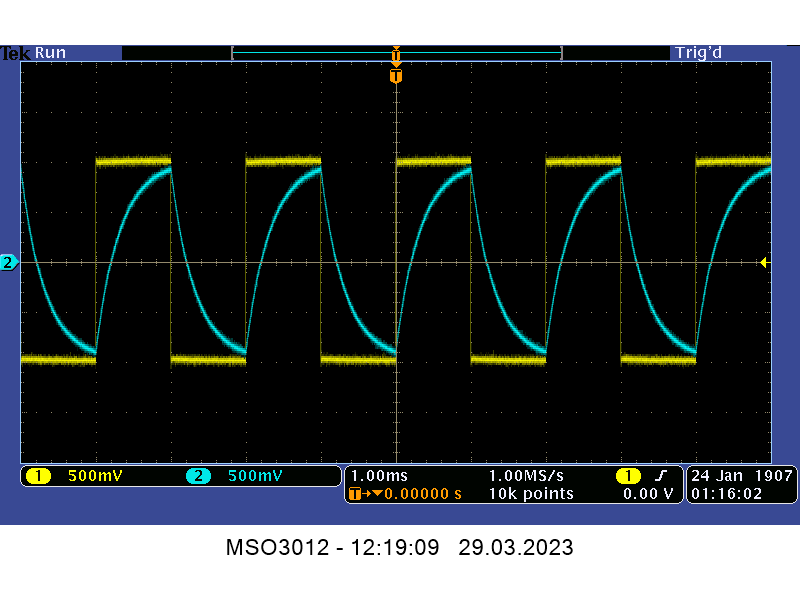
\includegraphics[scale=0.65]{RC-square-2ms}
\centering
\captionsetup{labelformat=empty}
\caption{Sygnał prostokątny \ \ $T = 2 \ ms \ \ \ f = 500 \ Hz$}
\end{figure}

\begin{figure}[H]
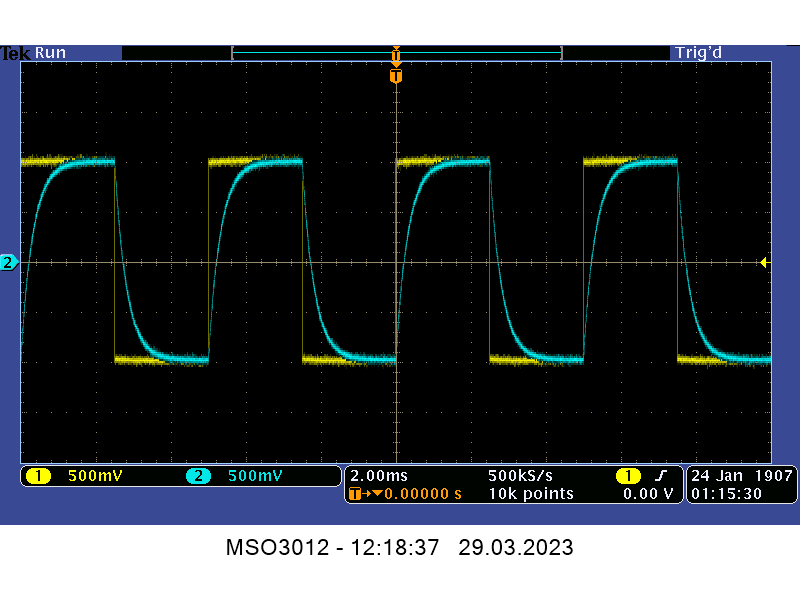
\includegraphics[scale=0.65]{RC-square-5ms}
\centering
\captionsetup{labelformat=empty}
\caption{Sygnał prostokątny \ \ $T = 5 \ ms \ \ \ f = 200 \ Hz$}
\end{figure}

\newpage
\paragraph{Ćwiczenie 2.3 \\}
Zbudowanie układu RLC (filtr środkowoprzepustowy), zmierzenie jego charakterstyk amplitudowej i fazowej dla sygnałów sinusoidalnych i wyzna- czenie jego częstotliwości rezonansowej.

\begin{figure}[H]
    \centering
    \subfloat[\centering ]{{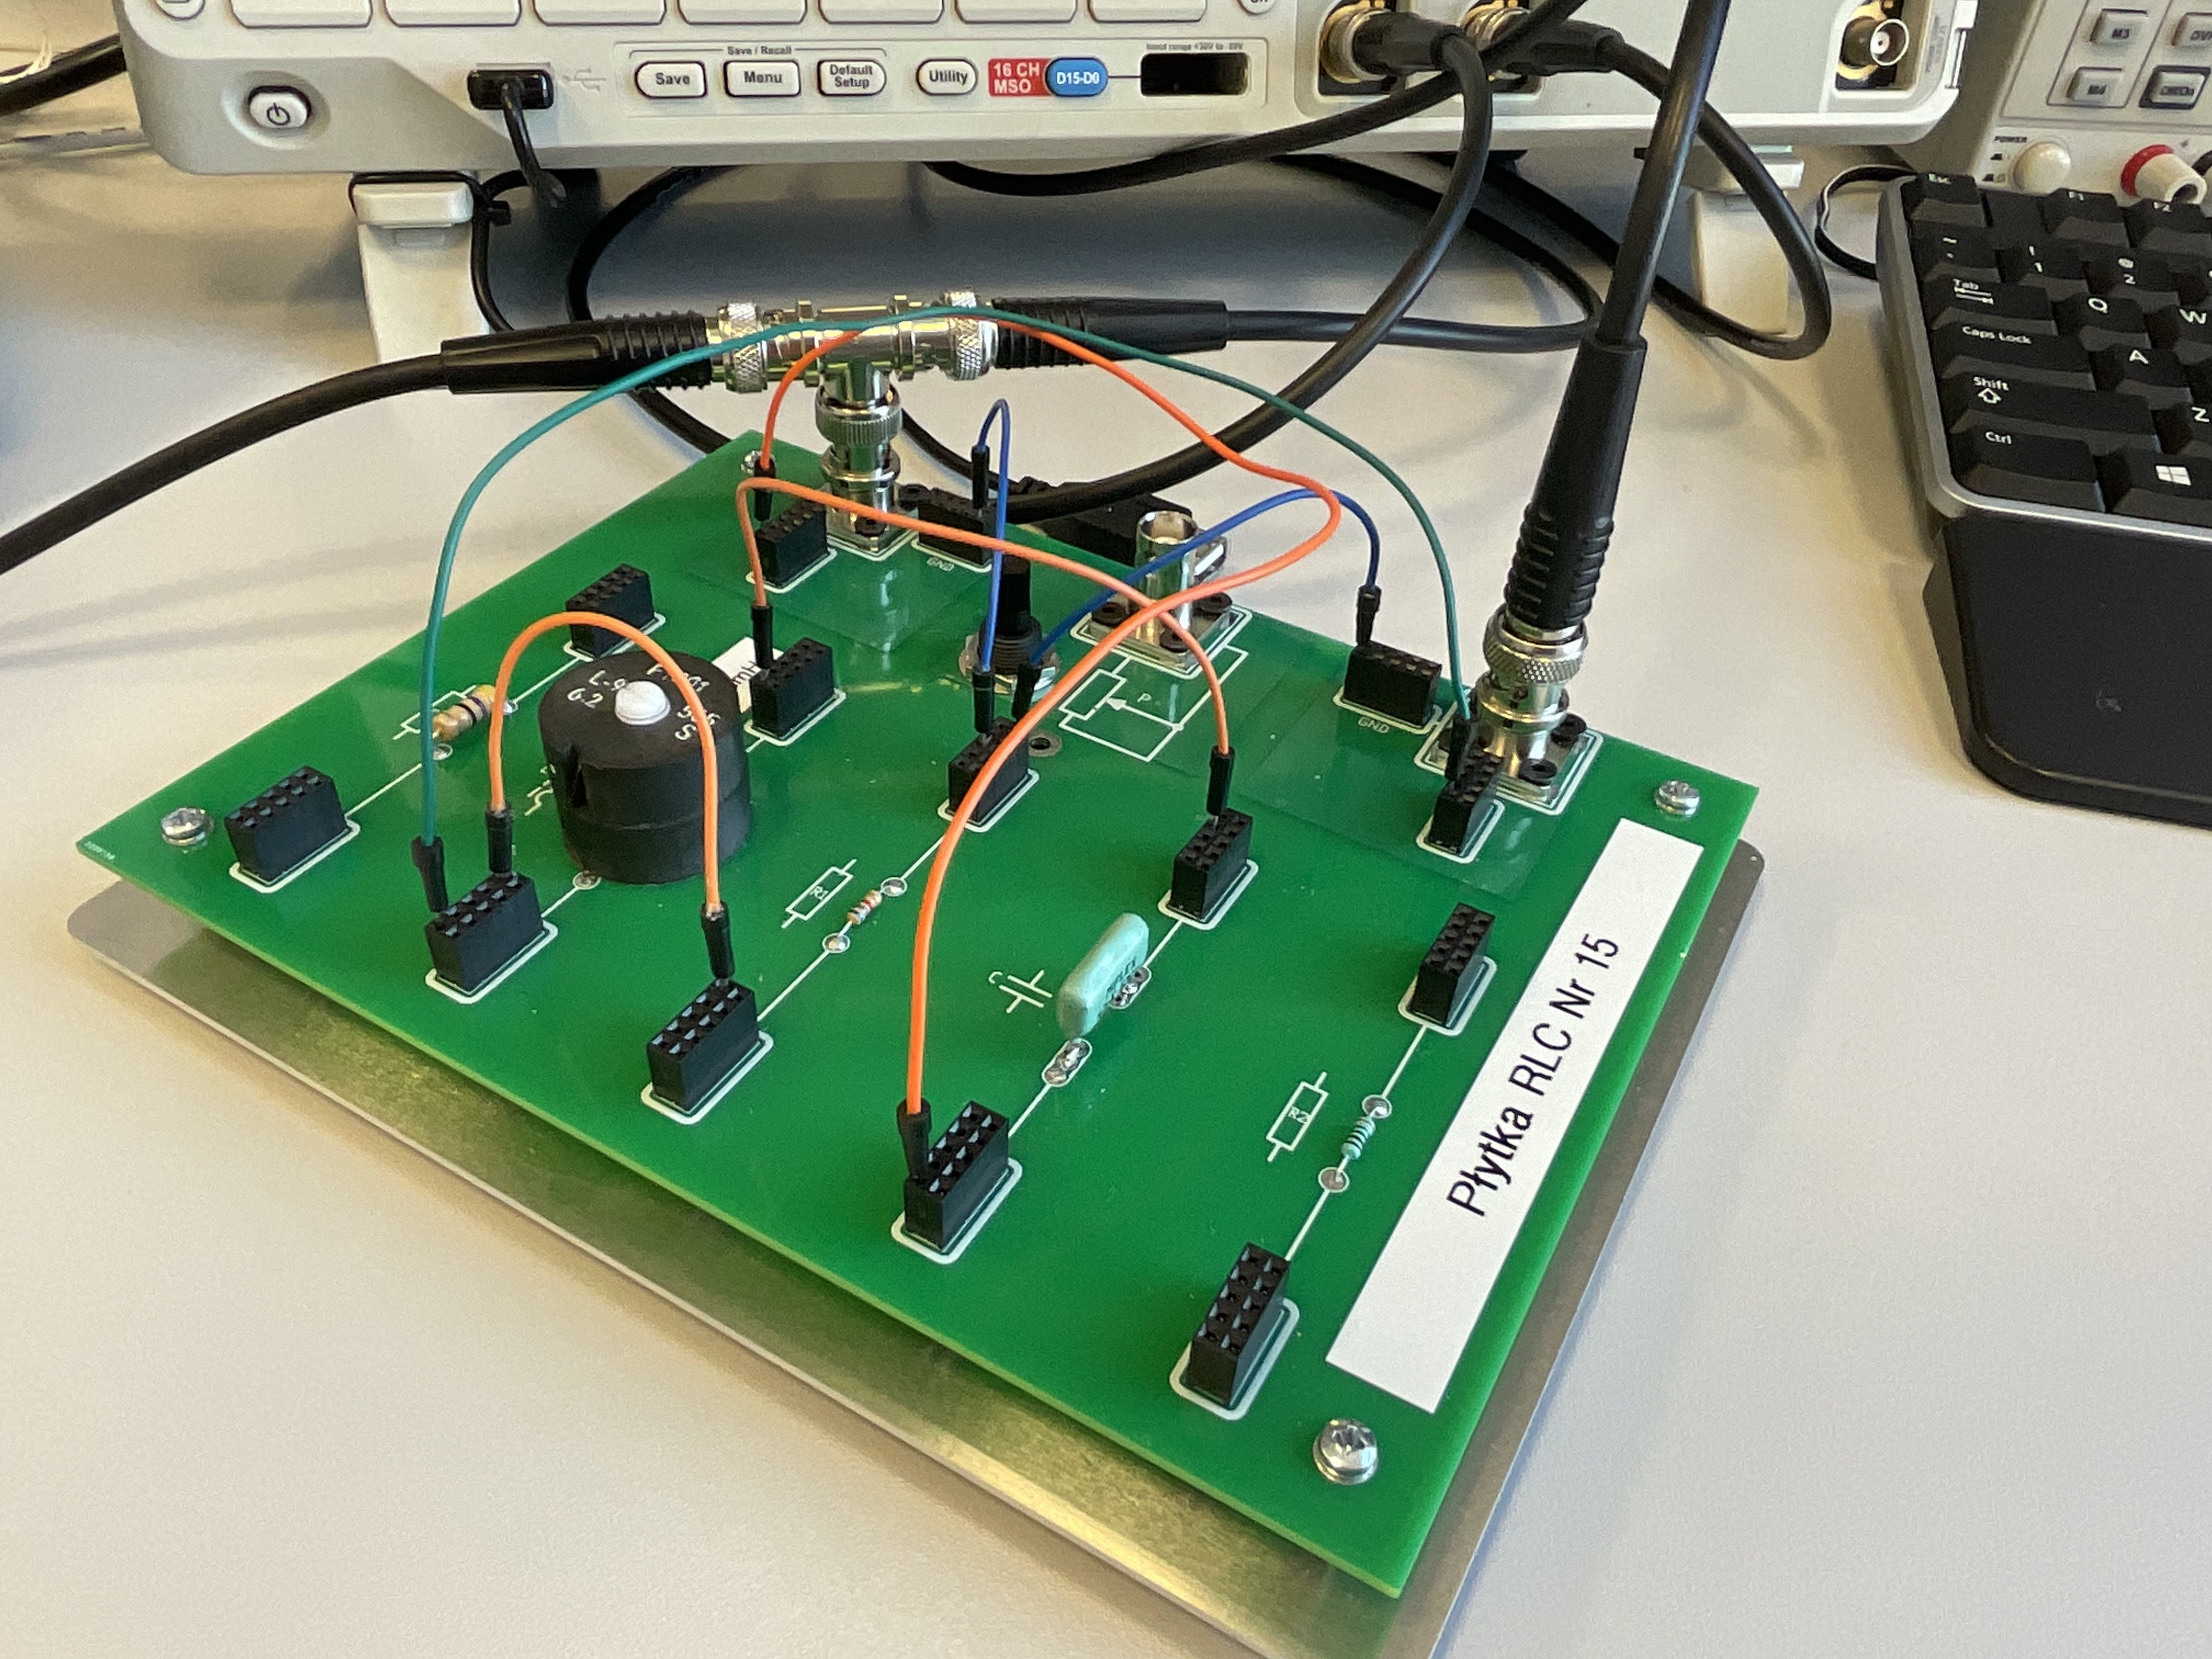
\includegraphics[width=7cm]{C4}}}%
    \qquad
    \subfloat[\centering ]{{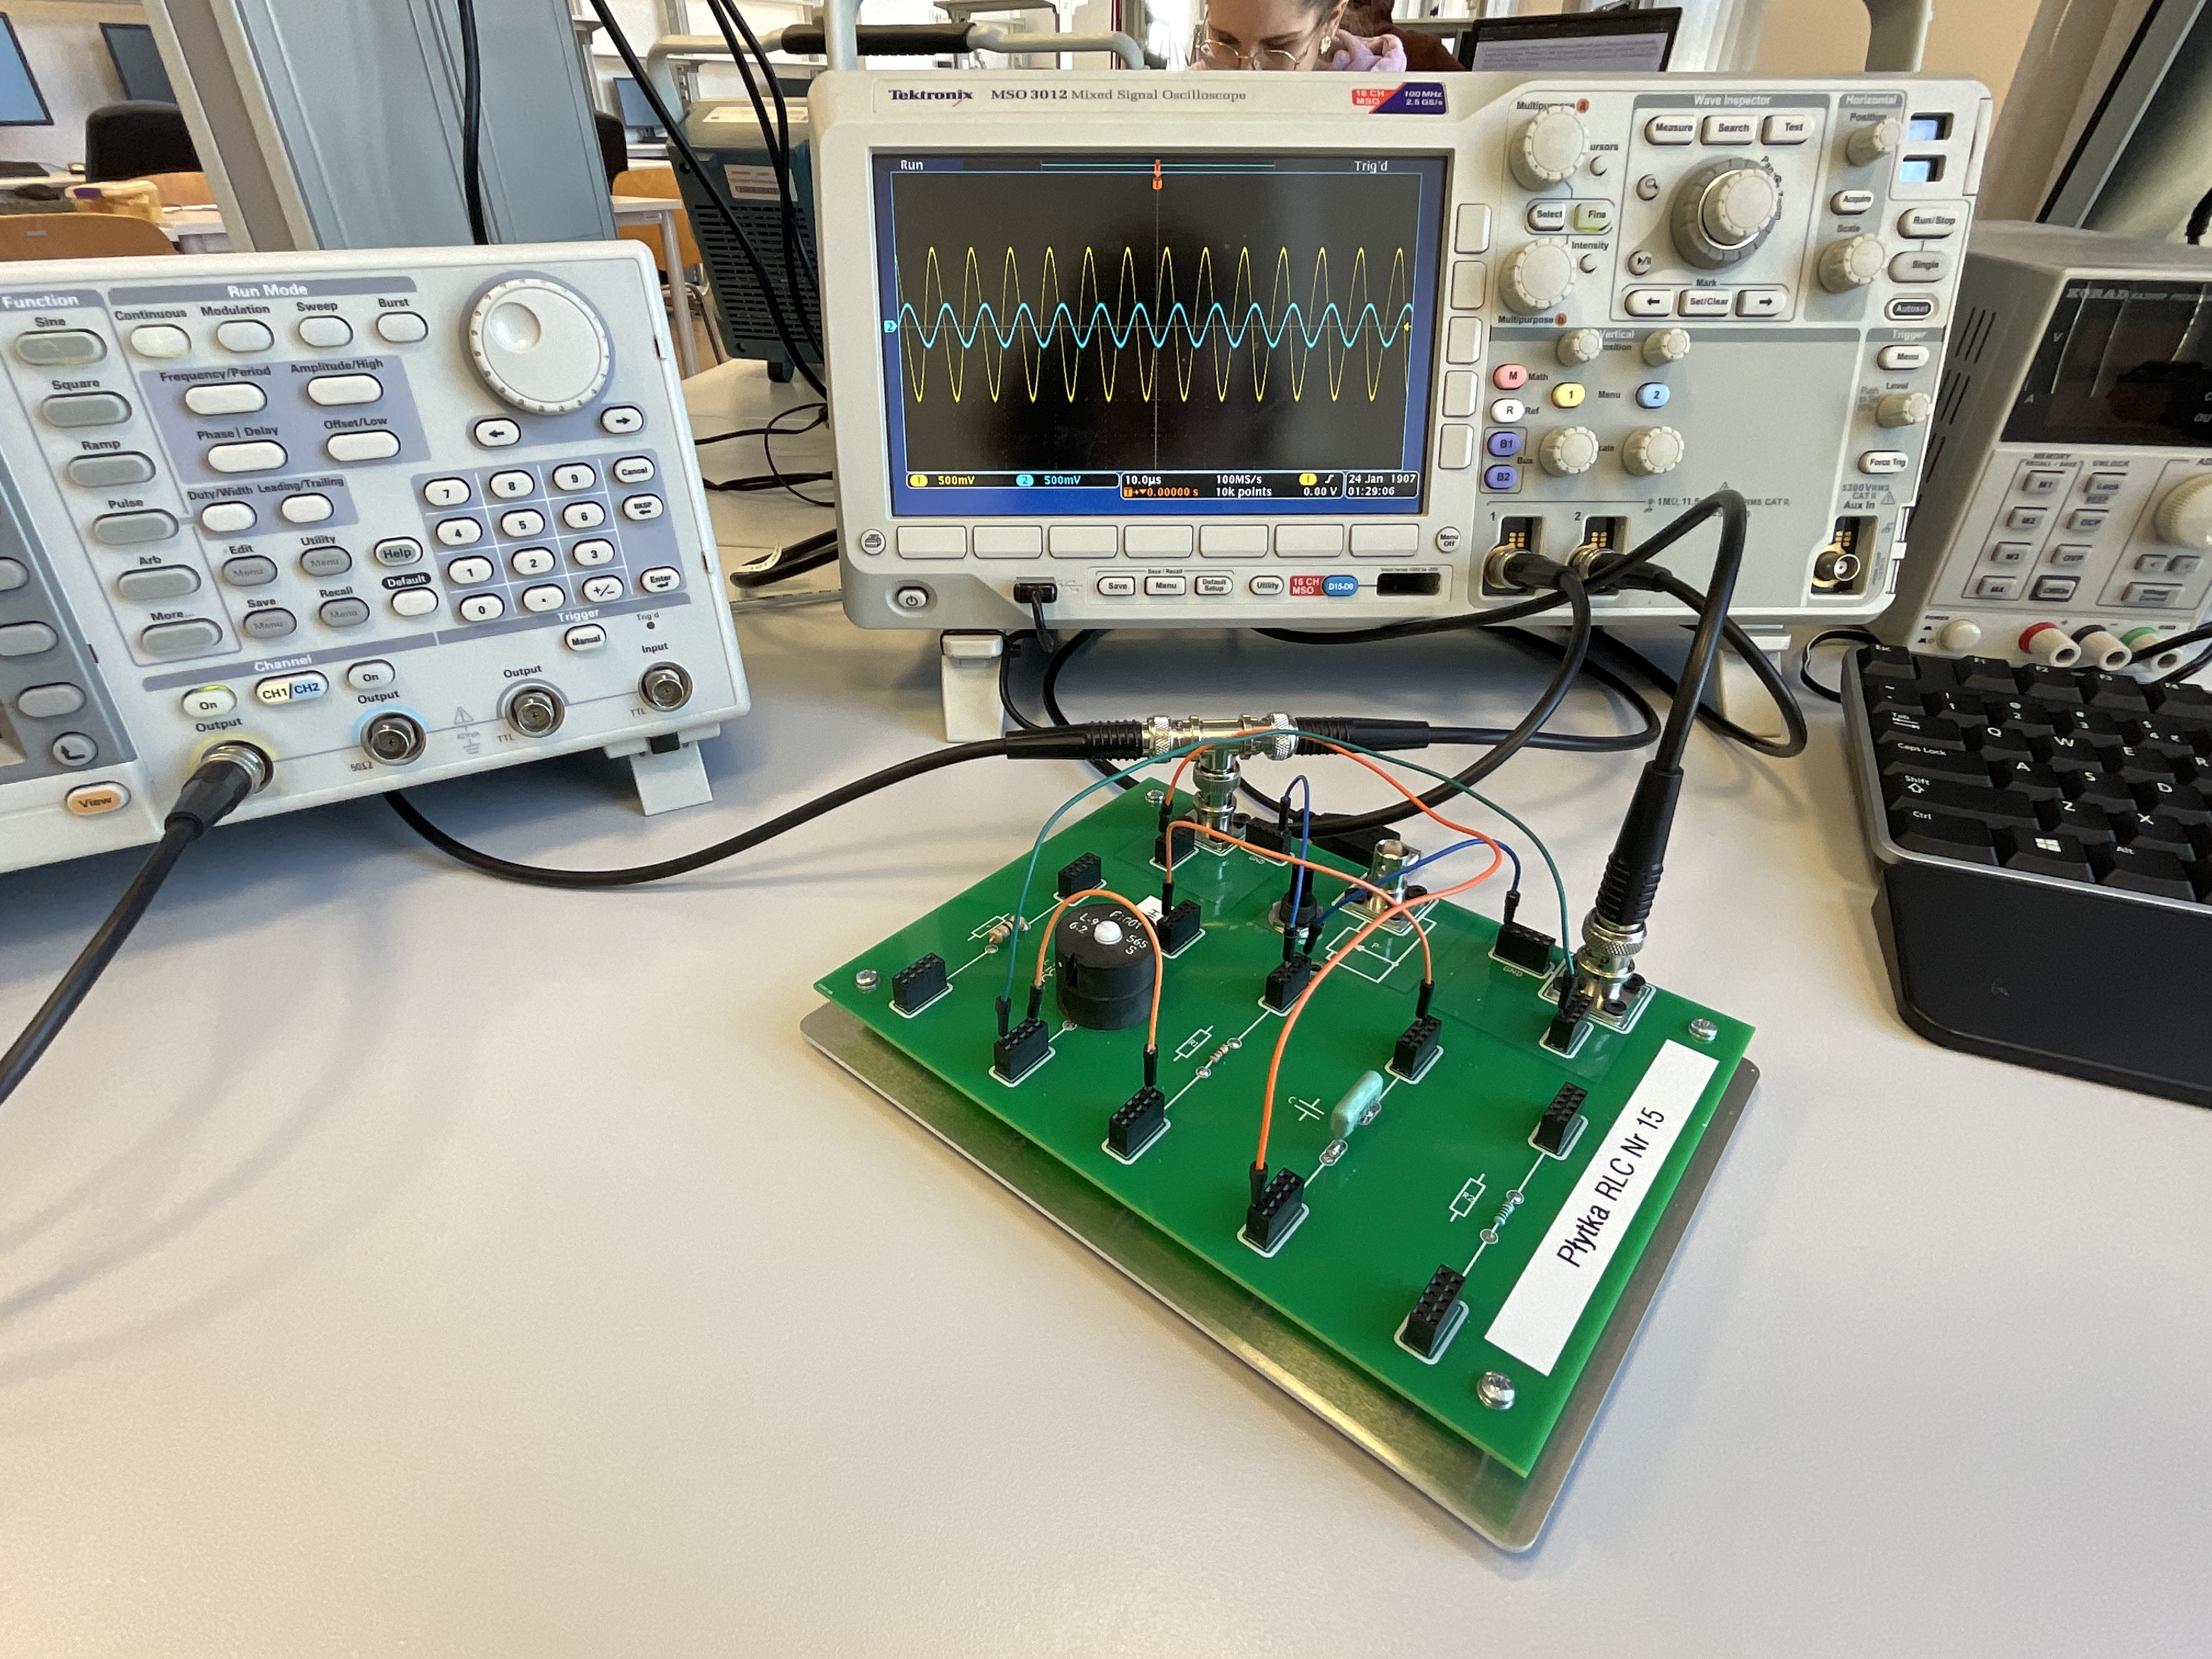
\includegraphics[width=7cm]{C5}}}%
\end{figure}

Montując układ RLC użyłem rezystora o oporze $6.8 \ k \Omega$, kondensatora o pojemności $47 \ nF$ i cewki o indukcyjności $15.8 \ mH$. Teoretyczna częstotliwość rezonansowa wynosi:

$$ f_r = \frac{1}{2 \pi \sqrt{LC}} = \frac{1}{2 \pi \sqrt{15.8 \cdot 47 \cdot 10^{-12}}} \left[ \frac{1}{s} \right] = 5840.4 \left[ Hz \right] $$

Podałem na wejście układu sygnał sinusoidalny o apmlitudzie $2 \ V$pp o częstotliwościach od $350 \ Hz$ do $120 kHz$. Wartości amplitudy wyjściowej oraz przesunięcia fazowego wynosiły jak w tabeli poniżej: \\
\\

\begin{tabular}{ | m{4cm} | m{4cm}| m{4cm} | m{3.5cm} | } 
  \hline
  \textbf{Częstotliwość} & \textbf{Amplituda wyjściowa} & \textbf{Przesunięcie fazowe} & \textbf{Stosunek } $U_{WY} / U_{WE}$ \\ 
  \hline
  $350 \ Hz$ & $1.14 \ V$ & $55.68^{\circ}$ & $0.57$ \\
  \hline
  $700 \ Hz$ & $1.58 \ V$ & $35.4^{\circ}$ & $0.79$ \\
  \hline
  $1.45 \ kHz$ & $1.86 \ V$ & $17.81^{\circ}$ & $0.93$ \\
  \hline
  $2.9 \ kHz$ & $1.96 \ V$ & $8.913^{\circ}$ & $0.98$ \\
  \hline
  $5.8 \ kHz$ & $2 \ V$ & $-0.5022^{\circ}$ & $1$ \\
  \hline
  $10 \ kHz$ & $1.96 \ V$ & $-6.805^{\circ}$ & $0.98$ \\
  \hline
  $20 \ kHz$ & $1.94 \ V$ & $-14.75^{\circ}$ & $0.97$ \\
  \hline
  $40 \ kHz$ & $1.84 \ V$ & $-36^{\circ}$ & $0.92$ \\
  \hline
  $80 \ kHz$ & $1.36 \ V$ & $-71.26^{\circ}$ &  $0.68$ \\
  \hline
  $120 \ kHz$ & $780 \ mV$ & $-97.39^{\circ}$ &  $0.39$ \\
  \hline
\end{tabular}

\newpage
Zamieszczam poniżej odczyty oscyloskopu. Kanał 1 (żółty) - sygnał wejściowy, kanał 2 (niebieski) - sygnał wyjściowy.

\begin{figure}[H]
    \centering
    \subfloat[\centering $350 \ Hz$]{{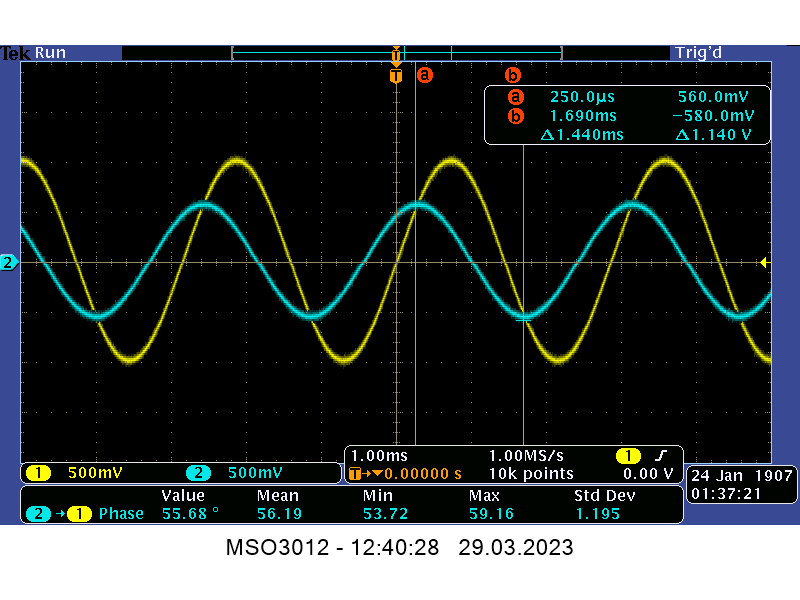
\includegraphics[width=7cm]{RLC-350-Hz}}}%
    \qquad
    \subfloat[\centering $700 \ Hz$]{{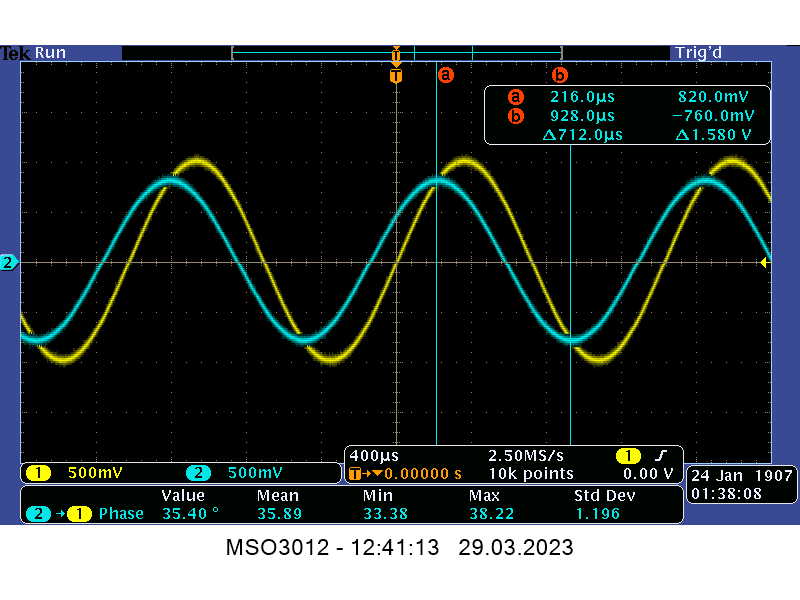
\includegraphics[width=7cm]{RLC-700-Hz}}}%
\end{figure}

\begin{figure}[H]
    \centering
    \subfloat[\centering $1.45 \ kHz$]{{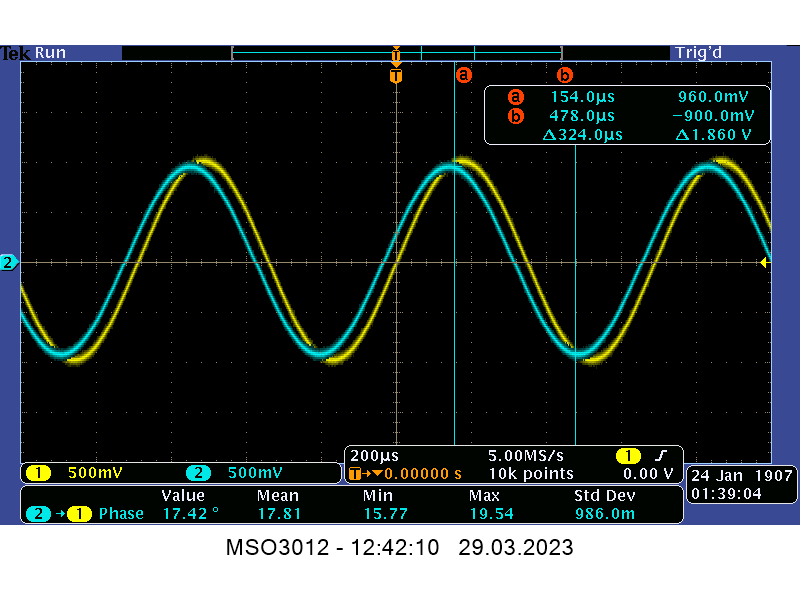
\includegraphics[width=7cm]{RLC-1_4-kHz}}}%
    \qquad
    \subfloat[\centering $2.9 \ kHz$]{{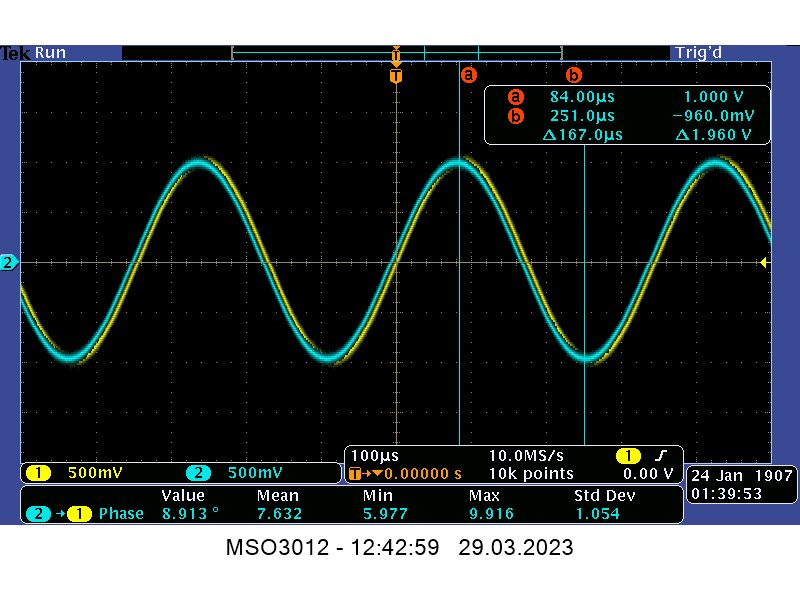
\includegraphics[width=7cm]{RLC-2_9-kHz}}}%
\end{figure}

\begin{figure}[H]
    \centering
    \subfloat[\centering $5.8 \ kHz$]{{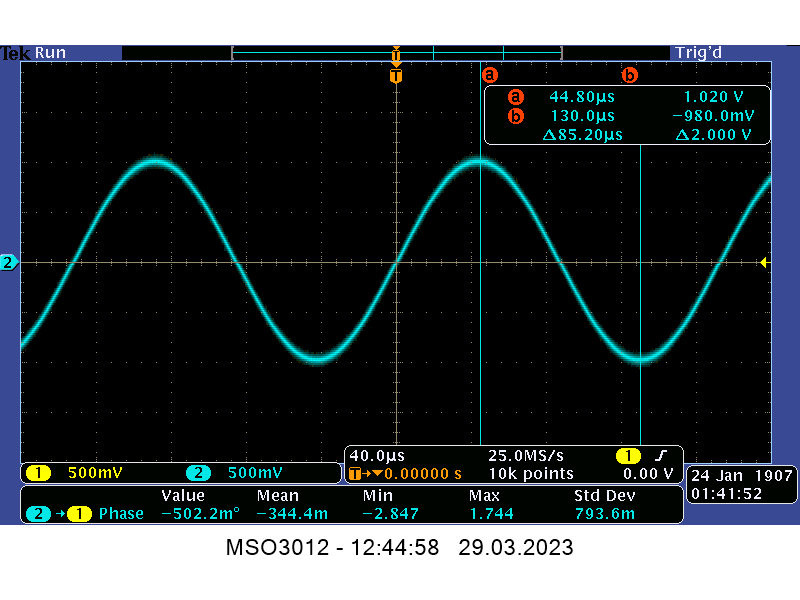
\includegraphics[width=7cm]{RLC-5_8-kHz}}}%
    \qquad
    \subfloat[\centering $10 \ kHz$]{{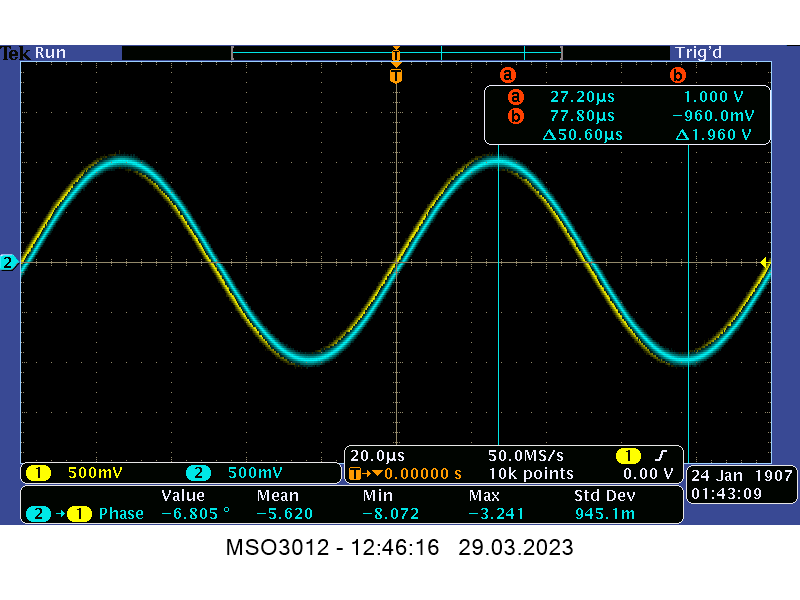
\includegraphics[width=7cm]{RLC-10-kHz}}}%
\end{figure}

\begin{figure}[H]
    \centering
    \subfloat[\centering $20 \ kHz$]{{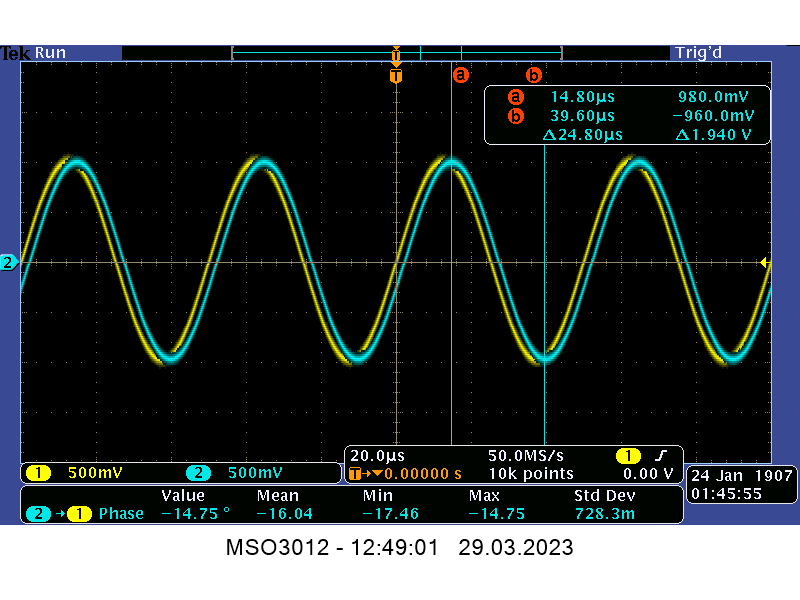
\includegraphics[width=7cm]{RLC-20-kHz}}}%
    \qquad
    \subfloat[\centering $40 \ kHz$]{{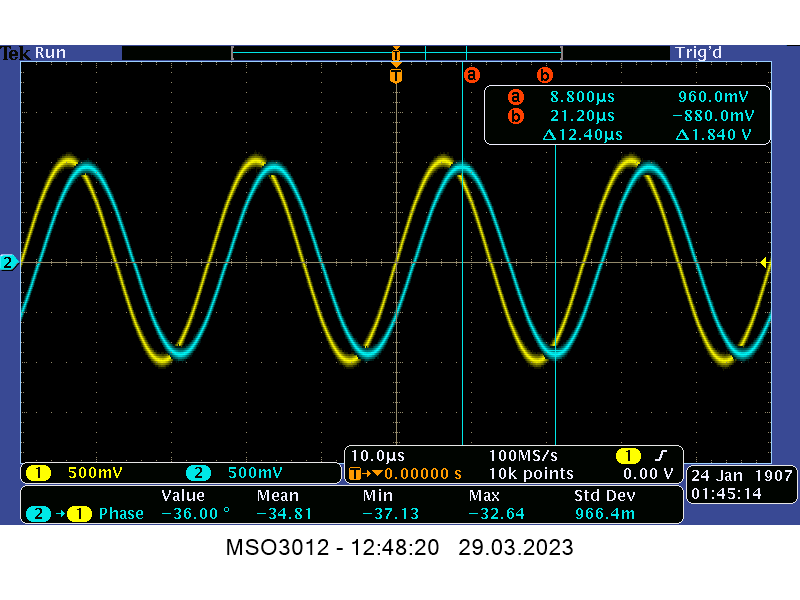
\includegraphics[width=7cm]{RLC-40-kHz}}}%
\end{figure}

\begin{figure}[H]
    \centering
    \subfloat[\centering $80 \ kHz$]{{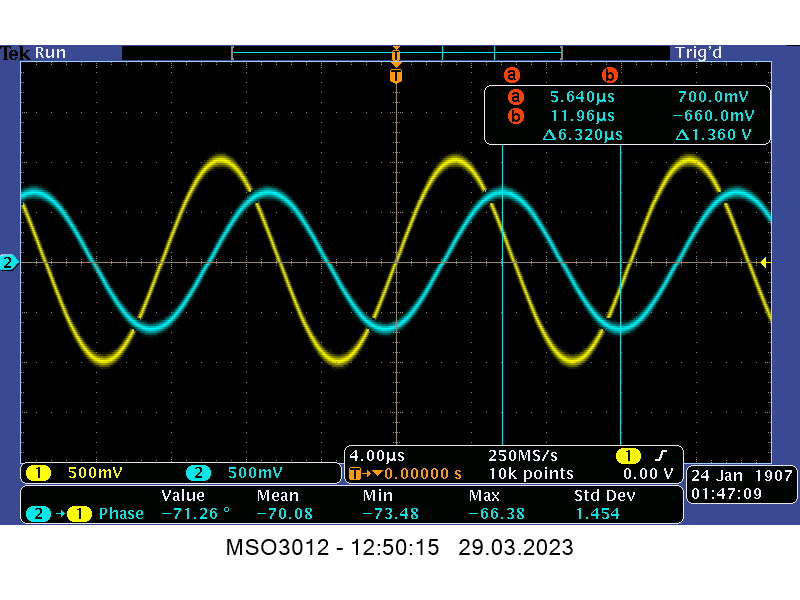
\includegraphics[width=7cm]{RLC-80-kHz}}}%
    \qquad
    \subfloat[\centering $120 \ kHz$]{{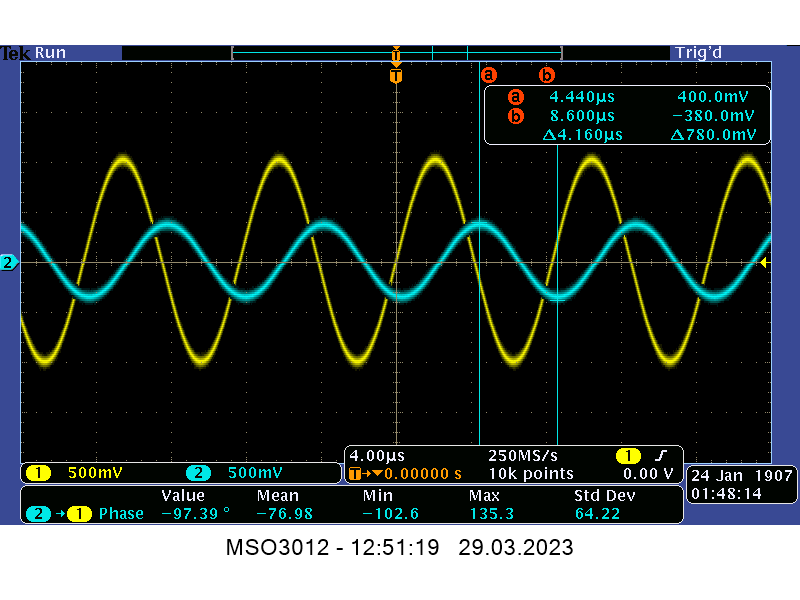
\includegraphics[width=7cm]{RLC-120-kHz}}}%
\end{figure}

\newpage
Wykresy: stosunek $U_{WY} / U_{WE}$ oraz przesunięcie fazowe w zależności od częstotliwości sygnału.

\begin{figure}[H]
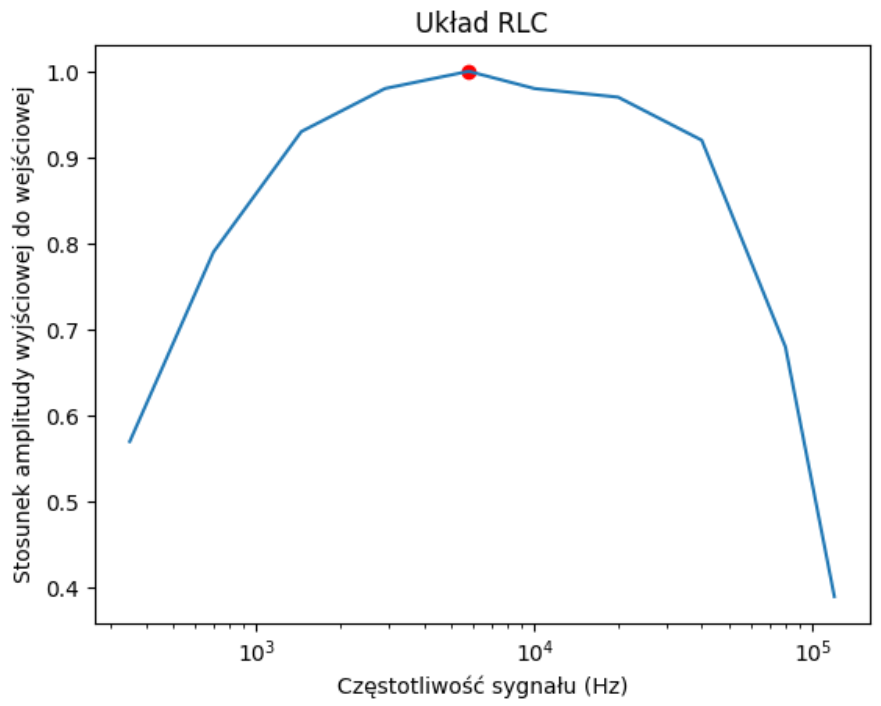
\includegraphics[scale=0.7]{D4}
\centering
\captionsetup{labelformat=empty}
\caption{}
\end{figure}

\begin{figure}[H]
\includegraphics[scale=0.7]{D5}
\centering
\captionsetup{labelformat=empty}
\caption{}
\end{figure}

\newpage
\paragraph{Omówienie wyników \\}
Na wykresach charakterystyk amplitudowych i fazowych filtrów zaznaczyłem czerwoną kropką punkty, w których powinno znajdować się miejsce częstotliwości odpowiednio granicznej górnej, granicznej dolnej i rezonansowej. \\

Dla charakterystyki amplitudowej filtrów górnoprzepustowego i dolnoprzepustowego jest to miejsce tłumienia większego niż $3 \ dB$. Wartość takiego stosunku amplitud wyjściowej do wejściowej można policzyć z definicji decybela:

$$ 20 \log_{10}(x) = -3 \Rightarrow x \approx 0.707 $$

Pozostałymi takimi punktami są $\frac{U_{WY}}{U_{WE}} = 1$ dla częstotliwości rezonansowej filtra środkowoprzepustowego i odpowiednio $45^{\circ}$, $-45^{\circ}$ i $0^{\circ}$ dla charakterystyk fazowych układów CR, RC i RLC. \\

Kropkami zielonymi zaznaczyłem te częstotliwości, które wyznaczyłem na podstawie sporządzonych wykresów. Są to odpowiednio: \\
$f_1 = 530 \ Hz \ \ \ f_2 = 525 \ Hz$ \\
$f_3 = 452 \ Hz \ \ \ f_4 = 490 \ Hz$ \\
$f_5 = f_6 = 5800 \ Hz$

Możemy obliczyć błędy względne:
$$ E_1 = \left| \frac{498 - 530}{498} \right| \approx 6.42\% $$
$$ E_2 = \left| \frac{498 - 525}{498} \right| \approx 5.42\% $$
$$ E_3 = \left| \frac{498 - 452}{498} \right| \approx 9.24\% $$
$$ E_4 = \left| \frac{498 - 490}{498} \right| \approx 1.61\% $$
$$ E_5 = E_6 = \left| \frac{5840 - 5800}{5840} \right| \approx 6.85\% $$

Błąd przy wyznaczaniu częstotliwości granicznych i rezonansowej to średnio około $6 \%$. \\

Także odpowiedzi układów CR i RC na sygnały prostokątne i trójkątne pokrywają się z teorią. Widać na podanych przeze mnie wyżej odczytach z oscyloskopu skąd biorą się nazwy "układ różniczkujący" i "całkujący". Widać też jaki wpływ na sygnał wyjściowy ma stała czasowa układów, które potrzebują $\tau$ czasu na powrócenie do stanu ustalonego.

\newpage
\paragraph{Notatki z zeszytu labolatoryjnego \\}
Poniżej załączone są notatki z zeszytu labolatoryjnego, które prowadziłem podczas zajęć wykonując pomiary.

\begin{figure}[H]
\includegraphics[scale=0.2]{B0}
\centering
\captionsetup{labelformat=empty}
\caption{}
\end{figure}

\begin{figure}[H]
\includegraphics[scale=0.2]{B1}
\centering
\captionsetup{labelformat=empty}
\caption{}
\end{figure}

\begin{figure}[H]
\includegraphics[scale=0.2]{B2}
\centering
\captionsetup{labelformat=empty}
\caption{}
\end{figure}

\begin{figure}[H]
\includegraphics[scale=0.2]{B3}
\centering
\captionsetup{labelformat=empty}
\caption{}
\end{figure}

\begin{figure}[H]
\includegraphics[scale=0.2]{B4}
\centering
\captionsetup{labelformat=empty}
\caption{}
\end{figure}

\end{document}